\section{Question Reduction}~\label{sec:introspection}
In this section, we give a proof for~\Cref{prop:QuestionReduction} by showing an algorithm that takes as input a synchronous CL verifier and transforms it into another synchronous CL verifier with a lower sampling complexity. Intuitively, this is done by asking both provers to sample their own question pairs for the $n$th game, and play the game based on the question pair they sampled. This procedure might first seem counter-intuitive, since the provers can always pre-select a question pair before the game  rather than sampling it honestly during the interaction. 

Roughly speaking, the verifier takes advantage of the entanglement shared between the provers to force them to sample a ``fresh" question pair for the given game. By leveraging self-testing techniques, the verifier can force the provers to make certain measurements on their entangled resources, thereby generating a question pair for the original game. 

The question reduction protocol consists of two components. The first component is the $n$-Pauli basis test. This is a subroutine that forces the provers to perform either an all $X$ or all $Z$ Pauli measurements on $n^{\alpha}$ EPR pairs, and we present this protocol in~\Cref{sec:Paulibasis}. The second component is the introspection test, where the verifier forces the provers to perform a specific set of measurements on the $n^{\alpha}$ EPR pairs, whereby the measurement outcomes are precisely the input distribution for the original game. 

\subsection{The magic square game}

\begin{figure}[!b]
	\begin{center}
		\begin{tabular}{|c|c|c|}
			\hline
			$x_1$ & $x_2$ & $x_3$ \\
			\hline 
			$x_4$ & $x_5$ & $x_6$ \\
			\hline
			$x_7$ & $x_8$ & $x_9$ \\
			\hline
		\end{tabular} 		\qquad
		\begin{tabular}{|c|c|c|}
			\hline
			$\cI_2 \otimes \rho^{Z}$ & $\rho^{Z} \otimes \cI_2$ & $\rho^{Z} \otimes \rho^{Z}$ \\
			\hline 
			$\rho^{X} \otimes \cI_2$ & $\cI_2 \otimes \rho^{Z}$ & $\rho^{X} \otimes \rho^{X}$ \\
			\hline
			$\rho^{X} \otimes \rho^{Z}$ & 	$\rho^{Z} \otimes \rho^{X}$ & $ - \left(\rho^{X}  \rho^{Z} \right) \otimes  \left(\rho^{X}  \rho^{Z} \right)$ \\
			\hline
		\end{tabular}
		
	\end{center}
	\caption{Left: The description for the magic square game, where each row and column corresponds to an equation. Right: A oracularizable perfect strategy for the magic square game.}
	\label{fig:magicsquare}
\end{figure}
We first introduce a key subroutine for the Pauli basis test, the Mermin-Peres magic square game~\cite{merminSimpleUnifiedForm1990, peresIncompatibleResultsQuantum1990}, in this subsection. We use the BCS formulation of this game as presented in~\cite{cleveCharacterizationBinaryConstraint2014}, where the game is defined by six equations and nine variables over $\bF_2$, where the variables are arranged on a three-by-three grid as presented in~\Cref{fig:magicsquare}. Every row and column in~\Cref{fig:magicsquare} corresponds to a constraint that multiplies to $1$, except for the last column, where the constraint multiplies to $-1$ instead. In this game, the referee randomly samples a constraint and a variable in the constraint and sends the constraint to one of the provers and the variable to the other prover. The prover must then respond with an assignment for their given constraint or variable. The provers win the game if their assignments are consistent with each other. If one of the provers is given an equation as the question, their assignment must also satisfy the constraint for the given equation. We also modify the magic square to be synchronous, meaning the verifier additionally samples a constraint or a variable with constant probability and sends it to both provers and expects the same answer in return.

The magic square game admits a perfect synchronous oracularizable strategy for both quantum models by using the measurement operator defined in~\Cref{fig:magicsquare}. In this strategy, the provers initially prepare two copies $\MEstate{2}$. In the event that the prover receives a variable, he measures the observable as displayed in the grid and returns the resulting eigenvalue (which is either $1$ or $-1$) as the assignment to the variable. If the prover receives an equation, he measures the observables for all three variables, returning the eigenvalue for each of the observables as the corresponding assignment for each of the variables. Since each observable on the grid commutes with all other observables that share a row or column with it, the order of measurement does not matter for the constraint question, and their measurement commutes on all possible question pairs, which implies that this perfect strategy is oracularizable. 


\subsection{The Pauli basis test} \label{sec:Paulibasis}
\jqnote{TODO: You need to change all the reference for~\cite{linTracialEmbeddableStrategies2024} to the correct ArXiv version once this is done.}

In this section, we recall the Pauli basis test. In this paper, we use the version of the Pauli basis test based on the elegant simplification given in~\cite{delasalleSpectralGapStability2022} and presented it similarly to~\cite[Section 6]{linTracialEmbeddableStrategies2024}. In comparison to the original Pauli basis test given in~\cite[Section 7]{jiMIPRE2022a}, this version does not rely on the low-individual degree test. Since this is a simple adaptation of the Pauli basis test, we present the protocol as is, and instead refer the reader to either~\cite{delasalleSpectralGapStability2022} or~\cite[Section 6]{linTracialEmbeddableStrategies2024} for more intuition.

%\jqnote{You need to use Justensen code~\cite[Fact 5.23]{bowenAldousLyonsConjectureII2024}, make sure that the runtime for encoding is actually $\poly(n)$, otherwise you have to just use the randomize result}
\jqnote{TODO, rewrite this, or move this to ~\cite{linTracialEmbeddableStrategies2024}}
Intuitively, the goal of the Pauli basis test is to force two honest provers to prepare $n$ copies of EPR pairs between them and measure either $(\rho^X)^{\tensor n}$ or $(\rho^Z)^{\tensor n}$ on their half of the EPR pair. For $n \in \bN$, we define the $n$ qubit Pauli basis test as the $\mu$-dependent Pauli basis test defined in~\cite[Section 6.3]{linTracialEmbeddableStrategies2024}, where $\mu$ is the uniform distribution over a subset $S^{\text{Paulibasis}}_n \subseteq \{0,1\}^n$ such that the spectral gap of $\mu$ is a constant.

We remark that the subset suggested in~\cite[Theorem 1.3]{delasalleSpectralGapStability2022} cannot be used directly in this context since it cannot be uniformly generated by a single circuit. Instead, recall in~\cite[Example 1.2]{delasalleSpectralGapStability2022}, given any $[k, n, d]$ binary linear code $C$, the code space for $C$, $S_{C} \subset \bF_{2}^n$, is a subset such that the uniform distribution of $S_C$ has a spectral gap of $\frac{2k}{d}$. Intuitively, any good binary linear code would lead to an efficient EPR tester. For any $n \in \bN$, consider the Justesen code~\cite{justesenClassConstructiveAsymptotically1972} with $R = \frac{\log(n)}{n}$, by definition this is a code with dimension $k = \lfloor \log(n) \rfloor$, length $n$ and distance $d \geq  0.11(n -  \log(n))$. Let $S^{\text{PB}}_n \subseteq\{0,1\}^n = \bF_2^n$ be the code space of the Justesen code mentioned above. Since the encoding map for the Justesen code can be implemented in $O(\poly(n))$ time, there exists an encoding map $\mathbf{\pi}^{\text{PB}}: \bN \times \{0,1\}^* \rightarrow \{0,1\}^*$ such that $\mathbf{\pi}^{\text{PB}} (n, s)$ is a bijection map that maps elements from $\{0,1\}^{\lfloor \log(n) \rfloor}$ to $S^{\text{PB}}_n$, with $\TIME_{\mathbf{\pi}^{\text{PB}}} (n) = \poly(n)$. Furthermore, the uniform distribution on $S^{\text{PB}}_n$ has a spectral gap of $\frac{2k}{d} \leq \frac{\log(n)}{0.11(n -  \log(n))} \leq 30$ for all $n$. Hence, it is sufficient to take $S^{\text{Paulibasis}}_n = S^{\text{PB}}_n$ in this context. 




We present the sample/decision procedure for the $n$-Pauli basis test in~\Cref{fig:PauliBasis}, and provide a diagram representation for the input distribution in~\Cref{fig:PauliBasisgraph}.  We recall the following rigidity theorem about the $n$ qubit Pauli basis test. 

%On a very high level, the honesty of the provers are enforced by periodically forcing one of the provers to make the same $\rho_X$ or $\rho_Z$ measurements on some subset of the $n$ copies and perform with the other prover who is asked to measure \textit{all} of the qubits. \cite{delasalleSpectralGapStability2022} realizes that the robustness of the Pauli basis test depends on the spectral gap of the probability in which the provers are asked to measure on these subsets. 



\begin{comment}
Recall by~\cite[proposition 1.3]{delasalleSpectralGapStability2022}, there exist a constant $C$ such that for every finite group $G$, there exist a subset, $S \subseteq G$ such that $|S| \leq C^{\text{spgap}} \log(|G|)$ where $C^{\text{spgap}}$ is a constant independent of the group such that the spectral gap\footnote{The definition of the spectral gap for a distribution of a group can be found in \cite[section 1.3]{delasalleSpectralGapStability2022}. For the purpose of this paper, this is a quantity which determine how good the EPR tester will be.} of the uniform distribution $S$ is a constant greater than 2. For every $n$, we represent the group $(\bZ_{2^n}, +)$ by elements of $\{0,1\}^n$ by the binary representation, and let $S^{\text{PB}}_n \subseteq\{0,1\}^n$ be the subset guarantee by the above proposition for the finite group $(\bZ_{2^n}, +)$. Since increasing the subset does not increase the spectral gap of the uniform distribution. By inserting more unique elements in into the original $S^{\text{PB}}$, we can, also without a lost of generality assume $\log{|S^{\text{PB}}_n|} \in \bN$ and $\log{|S^{\text{PB}}_n|} \leq \ceil{ \log(n + C^{\text{spgap}})}$. By definition, we have $|S^{\text{PB}}_n| = O(n) $ and $S^{\text{PB}}_n$ is also a subset of $\bF_{2^n}$ through the canonical encoding. 
\end{comment}


\begin{figure}[!b]
	\centering
	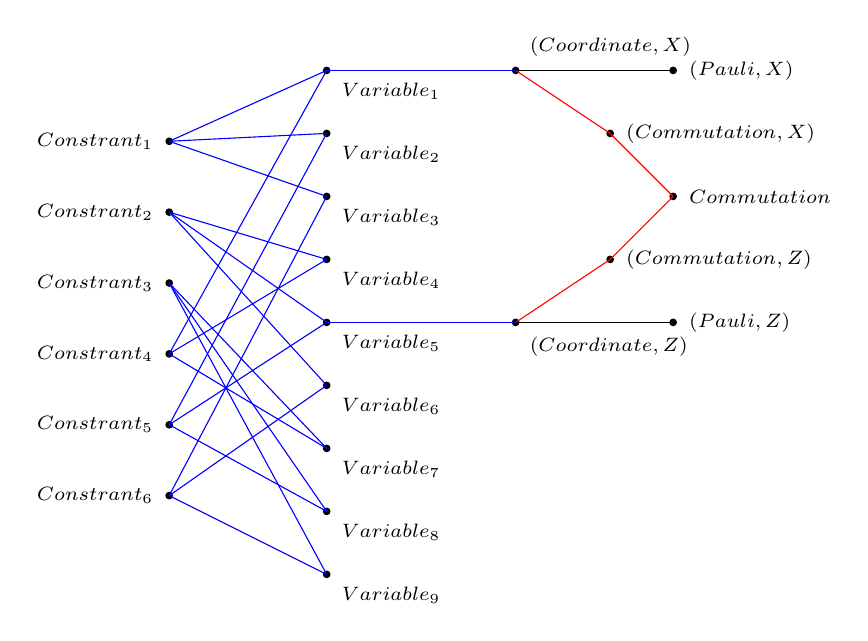
\begin{tikzpicture}[scale=.8]
		
		\tikzset{type/.style args={[#1]#2}{
				draw,circle,fill,scale=0.25,
				label={[font=\scriptsize, label distance=1pt]#1:#2}
		}}
		
		\foreach \i in {1,...,6} \draw (0,8-9/8*\i)
		coordinate (Constraint-\i)
		node[type={[180]$\text{Constrant}_\i$}] {};
		
		\foreach \i in {1,...,9} \draw (2.5,9-\i)
		coordinate (Variable-\i)
		node[type={[330]$\text{Variable}_\i$}] {};
		
		%\foreach \i in {6,...,9} \draw (2.5,9-\i)
		%coordinate (Variable-\i)
		%node[type={[330]$\text{Variable}_\i$}] {};
		
		
		\draw (5.5,8) coordinate (Cord-X) node[type={[45]$(\text{Coordinate},X)$}] {};
		\draw (5.5,4) coordinate (Cord-Z) node[type={[315]$(\text{Coordinate},Z)$}] {};
		
		\foreach \i in {1,...,3} \foreach \j in {1,...,3}
		\pgfmathsetmacro{\k}{(\i-1)*3+\j}
		\draw[blue] (Constraint-\i) -- (Variable-\k);
		
		\foreach \i in {4,...,6} \foreach \j in {1,...,3}
		\pgfmathsetmacro{\k}{\i-3+(\j-1)*3}
		\draw[blue] (Constraint-\i) -- (Variable-\k);
		\draw[blue] (Variable-1) -- (Cord-X);
		\draw[blue] (Variable-5) -- (Cord-Z);
		
		\draw (8,8) coordinate (Pauli-X) node[type={[0]$(\text{Pauli}, X)$}] {};
		\draw (8,4) coordinate (Pauli-Z) node[type={[0]$(\text{Pauli},Z)$}] {};
		\draw (8,6) coordinate (Commutation) node[type={[0]$\text{Commutation}$}] {};
		\draw (7,7) coordinate (Commutation-X) node[type={[0]$(\text{Commutation}, X)$}] {};
		\draw (7,5) coordinate (Commutation-Z) node[type={[0]$(\text{Commutation}, Z)$}] {};
		
		\foreach \from \to in {Cord-X/Commutation-X, Cord-Z/Commutation-Z,Commutation-Z/Commutation, Commutation-X/Commutation}
		\draw[red] (\from) -- (\to);
		\foreach \from \to in {Cord-X/Pauli-X, Cord-Z/Pauli-Z}
		\draw (\from) -- (\to);
	\end{tikzpicture}
	
	\caption{The typed graph $(\decidertypedtype^{\text{PB}}, \decidertypedquestionpair^{\text{PB}})$ for the $n$ qubit Pauli basis test, where each of the vertices above also contains a self-loop (this is a black edge). Similar to the definition of the CL distribution, each vertices in the graph represents a potential question label and each edge represents a potential question pair. Each of the edges are colour coded in order to better explain the game procedure and we refer to~\Cref{fig:PauliBasis} for more details. }
	\label{fig:PauliBasisgraph}
\end{figure}

\begin{figure}[!htbp]
	\centering
	\begin{gamespec}
		\setlength{\tabcolsep}{1em}
		\begin{tabularx}{\textwidth}{ l   l   X   }
			\toprule
			Question label & Question content & Answer format \\
			\midrule
			(Pauli,$W$) &  & $ t_{W} \in \{0,1\}^n$ \\
			(Coordinate, $W$)& $u_W \in S^{\text{PB}}_n$& $ t_{\text{(Pauli, W)}} \in \{0,1\}^{n}$ \\
			(Commutation, $W$)& $u_W \in S^{\text{PB}}_n$& $t_W  \in \{0,1\}$ \\
			Commutation& $(u_X,u_Z)  \in S^{\text{PB}}_n \times S^{\text{PB}}_n$& $(t_{X}', t_{Z}') \in \{0,1\}^{2n}$ \\
			$\text{Variable}_i$& $(u_X,u_Z) \in S^{\text{PB}}_n \times S^{\text{PB}}_n$& $t_{\text{var}} \in \{0,1\}$ \\
			$\text{Constraint}_i$& $(u_X,u_Z)\in S^{\text{PB}}_n \times S^{\text{PB}}_n$& $t_{\text{cons}} \in \{0,1\}^{3}$ \\
			\bottomrule
			\multicolumn{3}{c}{Figure: Q and A format for the $n$ qubit Pauli basis test, where $W\in \{X,Z\}$. }
		\end{tabularx}
		\begin{center}
			\textbf{Sampling procedure}
		\end{center}
		\begin{enumerate}
			\item Sample $(u_X,u_Z) \in S^{\text{PB}}_n \times S^{\text{PB}}_n$ uniformly at random. 
			\item Uniformly samples $(n_0, n_1) \in \decidertypedtype^{\text{PB}} \times \decidertypedtype^{\text{Paulibasis}}$, where $(\decidertypedtype^{\text{PB}},  \decidertypedquestionpair^{\text{PB}})$ is the graph in~\Cref{fig:PauliBasisgraph}, and perform rejection sampling until $(n_0, n_1) \in \decidertypedquestionpair^{\text{PB}}$. 
			\item Send the question label and question content corresponding to $n_0$ to one of the provers, and send the question content corresponding to the $n_1$ to the other prover.
		\end{enumerate}
		\begin{center}
			\textbf{Verification procedure}
			
		\end{center}
		\begin{itemize}
			\item (Self-loop): The provers win iff they output the same answer. 
			\item (Pauli, $W$) \textbf{--}  (Coordinate, $W$): Alice and Bob win iff $t_{W}|_{u_W} = t_{\text{(Pauli, W)}}|_{u_W}$. 
			\item  If $(n_0, n_1)$ are a red edge and $u_x \cdot u_z = 1$, the provers win if for the question label (Commutation, $W$) and (Commutation), the prover answers $0$, otherwise
			\begin{itemize}
				\item  (Coordinate, $W$)  \color{red} \textbf{--}   \color{black}  (Commutation, $W$): The provers win iff $u_W \cdot t_{\text{Pauli},W} = t_W$. 
				\item  (Commutation)  \color{red} \textbf{--}   \color{black}  (Commutation, $W$): The provers win iff $t_W = t_W'$. 
			\end{itemize}
			\item If $(n_0, n_1)$ are a blue edge and $u_x \cdot u_z = 0$, the provers wins if for the question label (Constraint, $i$) and (Variable, $j$), the prover answers $0$, otherwise:
			\begin{itemize}
				\item (Variable $1$)  \color{blue} \textbf{--}   \color{black}  (Coordinate, $X$): The provers iff $u_X \cdot t_X = t_{\text{var}}$.
				\item (Variable $5$)  \color{blue} \textbf{--}   \color{black}  (Coordinate, $Z$): The provers iff $u_Z \cdot t_Z = t_{\text{var}}$.
				\item (Constraint)  \color{blue} \textbf{--}  \color{black}   (Variable): The provers win iff $t_{\text{cos}}$ is consistent with the constraint in the magic square game, and $t_{\text{var}}$ is consistent with the assignment of $v_i$ within $t_{\text{cos}}$. 
			\end{itemize}
		\end{itemize}
		\vspace{1em}
	\end{gamespec}
	\caption{The description for the $n$ qubit Pauli basis test. Where $W \in \{X, Z\}$ in the decision procedure. }
	\label{fig:PauliBasis}
\end{figure}



\jqnote{TODO: I think this proof can be simplify for synchronous strategies, also to projectors are not trivial}
%\textbf{and $V_A (P) V_A^* = V_B (A^{op}) V_B^*$ for all $P \in \cA$}
\begin{theorem}[Rigidity for the $n$ qubit Pauli basis test] \label{thm:soundnessPaulibasis}
	Let $\cG^{\text{PB}}_n$ be the $n$ qubit Pauli basis test and let $\strategy = (\cL^2(\alicealg, \tau), \sigma \ket{\tau}, \{P_a^x \}_{x \in \cX})$ be a projective, tracially embeddable strategy such that $\omega(\cG^{\text{PB}}_n, \strategy) \geq 1 - \eps$. 
	\begin{comment}
	For $s \in \bF_{2^{n}}$, define the observables
	\begin{equation*}
		O^{\text{PB}, W}(u) = \sum_{q \in \bF_{2^n}} (-1)^{q \cdot u} P_s^{(\text{Pauli}, W)} \in \alicealg.
	\end{equation*}
	\end{comment}
	There exist two isometries $V_{A}: \cL^2(\alicealg, \tau) \rightarrow  \cL^2(\alicealg, \tau) \tensor \bC^{2^{2n}}$ and $V_{B}: \cL^2(\alicealg, \tau) \rightarrow \cL^2(\alicealg, \tau) \tensor \bC^{2^{2n}}$ with $( V_B \tensor \cI_{2^{2n}}) V_{A} =  V_{A} (V_B \tensor \bI_{2^{2n}})$ and a state $\ket{\text{Aux}} \in \cL^2(\alicealg, \tau) \otimes \bC^{2^{2n}}$ such that
	\begin{equation*} 
		\left\| \left(  V_B \tensor \cI_{2^{2n}}  \right) V_{A} \left(\sigma\ket{\tau}\right)  -\ket{\text{Aux}}  \ket{\text{ME}_2}^{\tensor n} \right\|^2 \leq O\left(\poly(\eps)\right),
	\end{equation*}
	and for all $W \in \{X, Z\}$ and $u \in \bF_{2^{n}}$
	\begin{align*} 
		&|  ((V_{A} P_s^{(\text{Pauli}, W)}  V_{A}^*)_{\alicealg A_1 A_2} \tensor (\cI_{2^{2n}} )_{B_1 B_2} - \\
		&\quad (\cI_{\cH})_{\alicealg} \otimes (\rho^{W}_s)_{A_1} \tensor (\cI_{2^{n}})_{A_2} \otimes  (\cI_{2^{2n}} )_{B_1 B_2} ) \ket{\text{Aux}}_{\alicealg A_2 B_2}  \MEstate{2}^{\tensor n}_{A_1 B_1}  |^2 \leq O\left(\poly(\eps )\right). \\
		&|  ((V_{B} (P_s^{(\text{Pauli}, W)})^{\text{op}}  V_{B}^*)_{\alicealg B_1 B_2} \tensor (\cI_{2^{2n}} )_{A_1 A_2} - \\
		&\quad (\cI_{\cH})_{\alicealg} \otimes (\rho^{W}_s)_{B_1} \tensor (\cI_{2^{n}})_{B_2} \otimes  (\cI_{2^{2n}} )_{A_1 A_2} ) \ket{\text{Aux}}_{\alicealg A_2 B_2}  \MEstate{2}^{\tensor n}_{A_1 B_1}  |^2 \leq O\left(\poly(\eps )\right). 
	\end{align*}

	\begin{comment}
			\begin{align*} 
			&|  ((V_{A} O^{(\text{PB}, W)} (u)  V_{A}^*)_{\alicealg A_1 A_2} \tensor (\cI_{2^{2n}} )_{B_1 B_2} - \\
			&\quad (\cI_{\cH})_{\alicealg} \otimes (\rho^{W}(u))_{A_1} \tensor (\cI_{2^{n}})_{A_2} \otimes  (\cI_{2^{2n}} )_{B_1 B_2} ) \ket{\text{Aux}}_{\alicealg A_2 B_2}  \MEstate{2}^{\tensor n}_{A_1 B_1}  |^2 \leq O\left(\poly(\eps )\right). \\
			&|  ((V_{A} O^{(\text{PB}, W)} (u)  V_{A}^*)_{\alicealg A_1 A_2} \tensor (\cI_{2^{2n}} )_{B_1 B_2} - \\
			&\quad (\cI_{\cH})_{\alicealg} \otimes (\rho^{W}(u))_{A_1} \tensor (\cI_{2^{n}})_{A_2} \otimes  (\cI_{2^{2n}} )_{B_1 B_2} ) \ket{\text{Aux}}_{\alicealg A_2 B_2}  \MEstate{2}^{\tensor n}_{A_1 B_1}  |^2 \leq O\left(\poly(\eps )\right). \\
			&|  (\left(V_{A} (O^{(\text{PB}, W)})^{\text{op}} (u)  V_{A}^*\right)_{\alicealg B_1 B_2} \tensor (\cI_{2^{2n}} )_{A_1 A_2} - \\
			&\quad (\cI_{\cH})_{\alicealg} \otimes (\rho^{W}(u))_{B_1} \tensor (\cI_{2^{n}})_{B_2} \otimes  (\cI_{2^{2n}} )_{A_1 A_2} ) \ket{\text{Aux}}_{\alicealg A_2 B_2}  \MEstate{2}^{\tensor n}_{A_1 B_1}  |^2 \leq O\left(\poly(\eps )\right).
		\end{align*}
	\end{comment}

	where the subscript $\alicealg$, $A_1$, $B_1$, $A_2$, $B_2$ and $\alicealg$ denotes the registers on which each operator acts (listed for clarity). 
\end{theorem}

%We remark that~\cite{linTracialEmbeddableStrategies2024} only shows it up to the observable level, but it can be proven for measurement operator by using a simple calculation in the case of $W(u)$ where $u = (1, \cdots,1)$.

The above rigidity follows from~\cite[Theorem 6.4]{linTracialEmbeddableStrategies2024} by defining $\mu$ as the uniform distribution of $S^{\text{PB}}_n$ as per the discussion above. We remark that in comparison to the $\mu$-dependent Pauli basis test defined in~\cite[Figure 3]{linTracialEmbeddableStrategies2024}, the sampling procedure for the $n$ qubit Pauli basis test is changed so that it is easier to show that the input distribution is samplable via a typed CL distribution. Although the anti-commutation test (the red vertices in~\Cref{fig:PauliBasisgraph}) within the $n$ qubit Pauli basis test is nine times more likely to occur than the commutation test (the blue vertices), the ratio between the likelihood of the two tests is still a constant. Furthermore, the question types (Variable 1), (Variable, 5), (Commutation, X), and (Commutation, Z) are added to ensure that there exists a perfect oracularizable strategy for the test. ~\Cref{thm:soundnessPaulibasis} still follows by modifying the inequality of the proof for~\cite[Lemma B.1]{linTracialEmbeddableStrategies2024} with a larger constant in the case where $u \cdot v = 0$, and changing equation (67) and (70) to incorporate the extra question labels added. 

%(\cite{jiMIPRE2022a} also added the same question type in their version of the Pauli basis test)

%The $V_A (P) V_A^* = V_B (A^{op}) V_B^*$ for all $P \in \cA$ condition follows from~\cite{linTracialEmbeddableStrategies2024} equation (43), where in the synchronous case, $V_A$ and $V_B$ are defined on the same representation, except $V_B$ is defined on the opposite algebra in the synchronous strategy case. 

In some sense, we can view~\Cref{thm:soundnessPaulibasis} as the ``soundness" condition about the Pauli basis test, since a $1 - \eps$ approximate strategy guarantees an approximate version of ``Pauli $X$ or Pauli $Z$ measurements on $n$-EPR pairs". In the following theorem, we show the ``completeness" and the ``runtime" condition related to the $n$ qubit Pauli basis test. 


%which intuitively correspond to the computational runtime for the verifier and ``completeness" condition. 
%We show the following basic properties about the $n$ qubit Pauli basis test.
\begin{theorem}[Properties of the $n$ qubit Pauli basis test] \label{thm:completenessPaulibasis}
	Let $\cG^{\text{PB}}_n$ be the $n$ qubit Pauli basis test
	\begin{enumerate}
		\item (Computation time): $\cG^{\text{PB}}_n$ is samplable via a $(\decidertypedtype^{\text{PB}}, \decidertypedquestionpair^{\text{PB}}, \{\decidertypedfunction^{v}\}_{v \in \decidertypedtype^{\text{PB}}} )$ typed CL distribution, where each $\decidertypedtype^{\text{PB}}: \bF_2^{2 \cdot s^{\text{SB}}_n} \rightarrow  \bF_2^{2 \cdot s^{\text{SB}}_n}$ is a first level CL function, where $s^{\text{SB}}_n = \lfloor \log(n) \rfloor$.  $\cG^{\text{PB}}_n$ has a decision complexity of $\poly(n)$. 
		\item (Completeness): There exists a perfect finite-dimensional symmetric oracularizable strategy $\strategy^{\text{PB}} = (\bC^{2^n} \otimes \bC^{2^n}, \MEstate{2}^{\otimes n} \otimes \MEstate{2}, \{P_a^x \})$ such that for all $s \in \{0,1\}^n$ and $W \in \{X,Z\}$
		\begin{equation*}
			 P_{s}^{(\text{Pauli}, W)} =  \rho^W_{s} \otimes \cI_2
		\end{equation*}
	\end{enumerate}
\end{theorem}
\begin{proof}
	% Note by the definition of $S^{\text{PB}}_n$, $s^{\text{SB}}\in \bN$. Hence, there exist a bijection $\mathbf{\pi}^{\text{PB}}_n: \{0,1\}^{s^{\text{SB}}_n}\rightarrow S^{\text{PB}}_n$ by some arbitrary indexing.
	For the remainder of this proof, we denote $W \in \{X,Z\}$.	Fix an integer $n\in \bN$. We first show that the $n$ qubit Pauli basis test is samplable via a typed CL distribution. Identify $\bF_2$ with $\{0,1\}$, and define each $\decidertypedfunction^v$ as follows: For every input $(s_{X}, s_{Z}) \in \{0,1\}^{s^{\text{SB}}_n} \times \{0,1\}^{s^{\text{SB}}_n}$, we define each of the linear function accordingly:
	\begin{itemize}
		\item  For $v \in \{ (\text{Pauli}, W), (\text{Coordinate}, W), (\text{Commutation}, W)\}$, 
		\begin{align*}
			\decidertypedfunction^{(\text{Pauli}, W)}(s_{X}, s_{Z}) &=  (0,0), \\
			\decidertypedfunction^{ (\text{Coordinate}, X)}(s_{X}, s_{Z}) = \decidertypedfunction^{ (\text{Commutation}, X)}(s_{X}, s_{Z}) &= (s_{X}, 0), \\
			\decidertypedfunction^{ (\text{Coordinate}, Z)}(s_{X}, s_{Z})  =\decidertypedfunction^{ (\text{Commutation}, Z)}(s_{X}, s_{Z}) &= (0, s_{Z}).
		\end{align*}
		\item Otherwise, $\decidertypedfunction^{v}$ is the identity function, or 
		\begin{equation*}
			\decidertypedfunction^{v}(s_{X}, s_{Z}) =  (s_{X}, s_{Z}). 
		\end{equation*}
	\end{itemize}
	
	For the decision process, given input $(u_{X}, u_{Z}) \in  S^{\text{PB}}_n \times S^{\text{PB}}_n$ and the output listed in the ``Answer format" from~\Cref{fig:PauliBasis}, the decision process for all the edges can be decided in $O(\poly(n))$ time since it involves either computing an inner product between elements of $\{0,1\}^n$ or some form of consistency test. Furthermore, since the map $\mathbf{\pi}^{\text{PB}}$ is computable uniformly in $O(\poly(n))$ time, the decider can compute each of the $(u_{X}, u_{Z})$ from $(s_{X}, s_{Z})$ sampled above. 
	%The only thing remaining is to check that the function $\mathbf{\pi}^{\text{PB}}_n$ can be computed in $\poly(n)$ time. To this end, since $s^{\text{SB}} = O(\log(n))$ by definition, any $\{0,1\}^{O(\log{n})} \rightarrow \{0,1\}^n$ function can be computed in $\poly(n)$ time, which implies that $\mathbf{\pi}^{\text{PB}}_n$ can be computed in $\poly(n)$ time.
	For the ``completeness" condition, we define the synchronous strategy $\strategy^{\text{PB}}$ over the Hilbert space $\bC^{2^n} \otimes \bC^{2^n}$ as follows: The joint state used between the two provers is $n$ EPR pairs, or $\MEstate{2}^{\otimes n} \otimes \MEstate{2}$. For $(u_X, u_Z) \in S^{\text{PB}}_n \times S^{\text{PB}}_n$, define
	\begin{equation*}
		\rho^{W}(u_W)_0 = \sum_{b \cdot u_W = 0} \rho^{W}_b, \qquad  \rho^{W}(u_W)_0 = \sum_{b \cdot u_W = 1}\rho^{W}_b,
	\end{equation*}
	and we see that
	\begin{equation*}
			\rho^{W}(u_W) = \rho^{W}(u_W)_0  - 	\rho^{W}(u_W)_1. 
	\end{equation*}
	We define the measurement operator $\{P^x_a\}$ for the symmetric strategy $\strategy^{\text{PB}}$ as
	\begin{align*}
		&P^{(\text{Pauli}, W)} = \rho^{W}_{t_W} \otimes \cI_2 &\text{ for all } t_W \in \{0,1\}^n, \\
		&P^{(\text{Coordinate}, W), u_{W}}_{ t_{\text{(Pauli, W)}}} = \sum_{ t_{\text{(Pauli, W)}}|_{u_{W}} = b}  \rho^{W}_b \otimes \cI_2  &\text{ for all }  t_{\text{(Pauli, W)}} \in \{0,1\}^n. \\
		&P^{(\text{Commutation, W}), (u_W) }_{t_W} = \rho^{W}(u_W)_{t_W} \otimes \cI_2 &\text{ for }  u_X \cdot u_Z = 0, t_W \in \{0,1\}\\
		&P^{(\text{Commutation}), (u_X, u_Z) }_{(t_W', t_Z')} = \left(\rho^{X}(u_X)_{t_X'}\right)\left( \rho^{Z}(u_Z)_{t_Z'}\right) \otimes \cI_2&\text{ for }  u_X \cdot u_Z = 0, t_W' \in \{0,1\}\\
		&P^{(\text{Commutation}), (u_X, u_Z) }_{a} = \begin{cases}
			\cI_{2^{n+1}} & \text{if } a= 0\\
			0 & \text{otherwise } \\
		\end{cases} & \text{ for } u_X \cdot u_Z = 1. \\
	& P^{(\text{Commutation, W}), (u_W) }_{a}  = \begin{cases}
		\cI_{2^{n+1}} & \text{if } a= 0\\
		0 & \text{otherwise } \\
	\end{cases} & \text{ for } u_X \cdot u_Z = 1. 
	\end{align*}
	For the magic square game, given $(u_X, u_Z)$ such that $u_x \cdot u_z = 1$, by \eqref{eq:genpaulicomm}, the observables $\rho^{X}(u_X)$ and  $\rho^{Z}(u_Z)$ anti-commutes. By applying~\cite[Theorem 7.11]{jiMIPRE2022a}, there exists a symmetric projective oracularizable strategy $\strategy^{\text{MS}} = (\bC^{2^{n+1}} \otimes \bC^{2^{n+1}}, \MEstate{2}^{\otimes n} \otimes \MEstate{2}, \{M_a^x \})$ such that for $b \in \{0,1\}$, 
	\begin{equation*}
		M_b^{(\text{Variable},1)} = \rho^{W}(u_W)_n \otimes \cI_2, \qquad M_b^{(\text{Variable},5)} = \rho^{W}(u_W)_n  \otimes \cI_2.
	\end{equation*}
	For $i \in \{2,3,4,6,7,8,9\}$, and $j \in \{1 ,\cdots, 6\}$,set 
	\begin{equation*}
		P_b^{(\text{Variable},i), (u_x, u_z)} = M_b^{(\text{Variable},i)}, \qquad P_b^{(\text{Constraint},j), (u_x, u_z)} = M_b^{(\text{Constraint},j)}. 
	\end{equation*}
	In the event that  $u_x \cdot u_z = 0$, set 
	\begin{equation*}
		P_b^{(\text{Variable},i), (u_x, u_z)} = P_b^{(\text{Constraint},j), (u_x, u_z)} = \begin{cases}
			\cI_{2^{n+1}} & \text{if } b= 0\\
			0 & \text{otherwise } \\
		\end{cases}. 
	\end{equation*}
	Since all measurement operators $\strategy^{\text{PB}}$ are defined within $\bigotimes_{i = 0}^{n+1} \cM_2(\bC)$, for all $a \in \cA$
	\begin{equation*}
		\left(P_{a} \otimes \cI_{\mathbf{B}} \right) \MEstate{2}^{\otimes n}_{\mathbf{AB}} \otimes \MEstate{2}_{\mathbf{AB}}  = \left( \cI \otimes P_{a}^{T} \right) \MEstate{2}^{\otimes n}_{\mathbf{AB}} \otimes \MEstate{2}_{\mathbf{AB}}
	\end{equation*}
	 for all measurements within $\strategy^{\text{PB}}$. We now verify that $\strategy^{\text{PB}}$ is indeed an oracularizable and perfect strategy by considering all possible question pairs in $\cG^{\text{PB}}_n$. 
	\begin{itemize}
		\item (Self-loop) Since all the measurements are projective, this is trivially true. 
		\item (Pauli, $W$) \textbf{--}  (Coordinate, $W$)  This follows since both question labels require a measurement in the $W$ basis. 
		\item  If $u_x \cdot u_z = 0$
		\begin{itemize}
			\item The red-edge question pairs are trivially perfect/oracularizable, since one of the measurement operators is always the identity. 
			\item  (Coordinate, $W$)  \color{red} \textbf{--}   \color{black} (Commutation, $W$): This follows since both question labels require a measurement in the $W$ basis. 
			\item  (Commutation)  \color{red} \textbf{--}   \color{black}  (Commutation, $W$): By~\eqref{eq:genpaulicomm}, $\rho^{X}(u_X)$ commutes with $\rho^{Z}(u_Z)$. Hence, $\{ \rho^{X}(u_X)_i\}_{i \in \{0,1\}}$ pairwise commute with $\{ \rho^{Z}(u_Z)_i\}_{i \in \{0,1\}}$, and the statement follows accordingly. 
		\end{itemize}
		\item If $u_x \cdot u_z = 1$
		\begin{itemize}
			\item The blue edge question pairs are trivially perfect/oracularizable, since one of the measurement operators is always the identity. 
			\item (Variable $1$)  \color{blue} \textbf{--}   \color{black}  (Coordinate, $X$):  This follows since both question labels require a measurement in the $X$ basis. 
			\item (Variable $5$)  \color{blue} \textbf{--}   \color{black}  (Coordinate, $Z$):  This follows since both question labels require a measurement in the $Z$ basis. 
			\item (Constraint)  \color{blue} \textbf{--}  \color{black}   (Variable): This follows by~\cite[Theorem 7.11]{jiMIPRE2022a}.
		\end{itemize}
		This shows that $\strategy^{\text{PB}}$ is a symmetric oracularizable strategy.
	\end{itemize}
\end{proof}

 %We remark that since $\cG^{\text{PB}}_n$ are synchronous, the strategy which arises from the completeness condition are also synchronous.

\subsection{The Introspection protocol} \label{sec:introspectionprotocol}

\begin{comment}
	
	
	As a simple example, the verifier can force one of the prover, Alice, to make a $Z$-measurement on one of her shared EPR bits in order to sample a bit from the seed of a CL distribution. In this case, the other prover, Bob,  also make can make a $Z$-measurement in the same location Alice has on his half of the EPR pair in order to sample the same bits Alice has. In the event that Bob should not get that bit of the seed (i.e. the bit is in the Null space of Bob's CL function), the verifier can force Bob to make an $X$-measurement on his half of the EPR bits, thereby making it unentangled to Alice's half, which prevents him from knowing which bit Alice samples. As we see later in this section, the distribution $\mu$ being a CL distribution plays a critical role in the question reduction protocol. 
	
\end{comment}

In this subsection, we present the introspection protocol for a game that is CL samplable, which provides the algorithm  $\texttt{QuestionReduction}_{\alpha, k}$ required in~\Cref{prop:QuestionReduction}. For $\alpha, n \in \bN$, and a CL samplable game $\cG = (\cX, \cA, \mu, D)$, where the question distribution $\mu$ is a $(k,m,p)$ CL distribution with $m \cdot p \leq n^{\alpha}$, we define the sampling procedure for the $(\cG,\alpha, k)$-introspection protocol in~\Cref{fig:Introspectionsample}, the verification procedure in~\Cref{fig:Introspectionverification}, and a typed graph for the input distribution in~\Cref{fig:Introspectiongraph}. We remark that the introspection protocol is almost the same as the one presented in~\cite[Figure 10]{jiMIPRE2022a}, with minor adjustments for clarity. 

%(mainly the generalized Pauli question $(\text{Gen Pauli}, W)$ for $W \in \{X,Z\}$). 


\begin{figure}[!t]
	\centering
	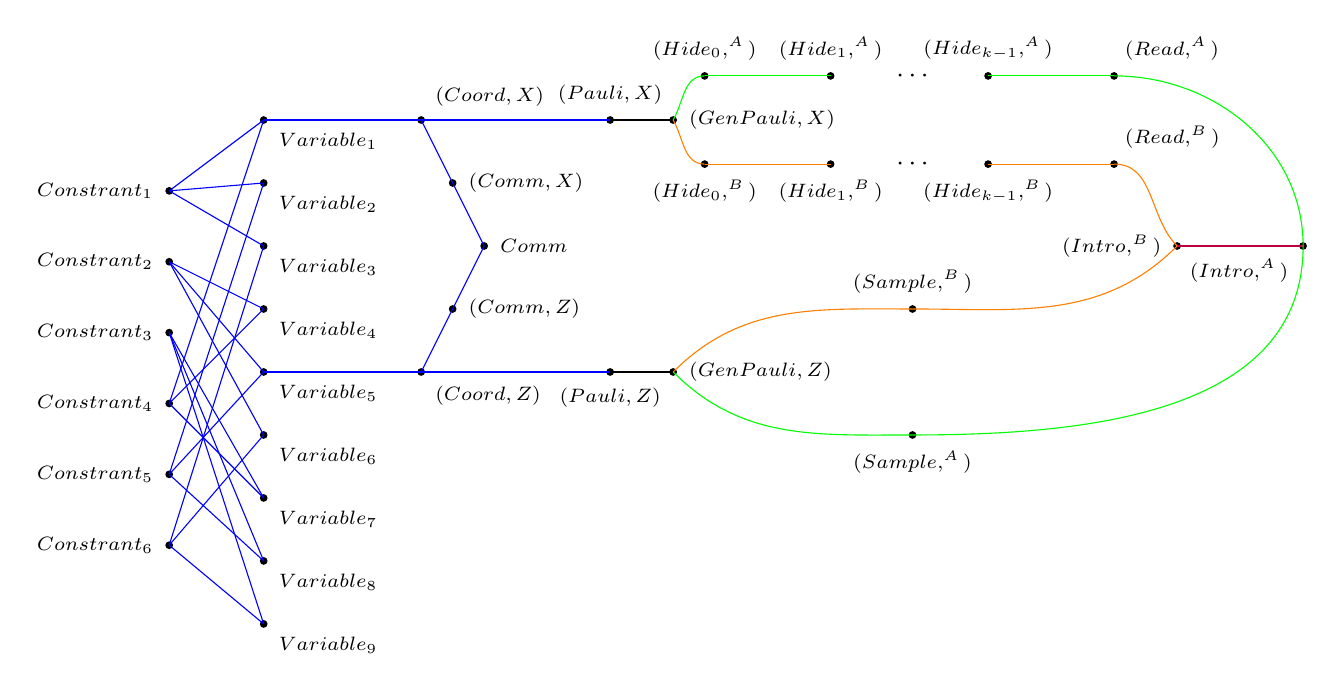
\begin{tikzpicture}[scale=.8]
		
		\tikzset{type/.style args={[#1]#2}{
				draw,circle,fill,scale=0.25,
				label={[font=\scriptsize, label distance=1pt]#1:#2}
		}}
		
		\foreach \i in {1,...,6} \draw (0,8-9/8*\i)
		coordinate (Constraint-\i)
		node[type={[180]$\text{Constrant}_\i$}] {};
		
		\foreach \i in {1,...,9} \draw (1.5,9-\i)
		coordinate (Variable-\i)
		node[type={[330]$\text{Variable}_\i$}] {};
		
		%\foreach \i in {6,...,9} \draw (2.5,9-\i)
		%coordinate (Variable-\i)
		%node[type={[330]$\text{Variable}_\i$}] {};
		
		
		\draw (4,8) coordinate (Cord-X) node[type={[45]$(\text{Coord},X)$}] {};
		\draw (4,4) coordinate (Cord-Z) node[type={[315]$(\text{Coord},Z)$}] {};
		
		
		\foreach \i in {4,...,6} \foreach \j in {1,...,3}
		\pgfmathsetmacro{\k}{\i-3+(\j-1)*3}
		\draw[blue] (Constraint-\i) -- (Variable-\k);
		\draw[blue] (Variable-1) -- (Cord-X);
		\draw[blue] (Variable-5) -- (Cord-Z);
		
		\draw (7,8) coordinate (Pauli-X) node[type={[90]$(\text{Pauli}, X)$}] {};
		\draw (7,4) coordinate (Pauli-Z) node[type={[270]$(\text{Pauli},Z)$}] {};
		\draw (5,6) coordinate (Commutation) node[type={[0]$\text{Comm}$}] {};
		\draw (4.5,7) coordinate (Commutation-X) node[type={[0]$(\text{Comm}, X)$}] {};
		\draw (4.5,5) coordinate (Commutation-Z) node[type={[0]$(\text{Comm}, Z)$}] {};
		
		\foreach \from \to in {Cord-X/Commutation-X, Cord-Z/Commutation-Z,Commutation-Z/Commutation, Commutation-X/Commutation}
		\draw[blue] (\from) -- (\to);
		\foreach \from \to in {Cord-X/Pauli-X, Cord-Z/Pauli-Z}
		\draw[blue] (\from) -- (\to);
		\foreach \i in {1,...,3} \foreach \j in {1,...,3}
		\pgfmathsetmacro{\k}{(\i-1)*3+\j}
		\draw[blue] (Constraint-\i) -- (Variable-\k);
		
		\draw (8,8) coordinate (GPauli-X) node[type={[0]$(\text{Gen Pauli}, X)$}] {};
		\draw (8,4) coordinate (GPauli-Z) node[type={[0]$(\text{Gen Pauli},Z)$}] {};
		\foreach \from \to in {GPauli-X/Pauli-X, GPauli-Z/Pauli-Z}
		\draw(\from) -- (\to);
		
		
		\draw (8.5,8.7) coordinate (Hide-1-A) node[type={[90]$(\text{Hide}_0, \decidertypedfunction^{A})$}] {};
		\draw (10.5,8.7) coordinate (Hide-2-A) node[type={[90]$(\text{Hide}_1, \decidertypedfunction^{A})$}] {};
		\draw (11.8,8.7) node {$\cdots$};
		\draw (13,8.7) coordinate (Hide-k-A) node[type={[90]$(\text{Hide}_{k-1}, \decidertypedfunction^{A})$}] {};
		\draw (15,8.7) coordinate (Read-A) node[type={[80]$(\text{Read},  \decidertypedfunction^{A})$}] {};
		
		\draw (8.5,7.3) coordinate (Hide-1-B) node[type={[270]$(\text{Hide}_0, \decidertypedfunction^{B})$}] {};
		\draw (10.5,7.3) coordinate (Hide-2-B) node[type={[270]$(\text{Hide}_1, \decidertypedfunction^{B})$}] {};
		\draw (11.8,7.3) node {$\cdots$};
		\draw (13,7.3) coordinate (Hide-k-B) node[type={[270]$(\text{Hide}_{k-1}, \decidertypedfunction^{B})$}] {};
		\draw (15,7.3) coordinate (Read-B) node[type={[80]$(\text{Read},  \decidertypedfunction^{B})$}] {};		
		
		
		\draw (16,6) coordinate (Intro-B) node[type={[180]$(\text{Intro},  \decidertypedfunction^{B})$}] {};
		\draw (18,6) coordinate (Intro-A) node[type={[215]$(\text{Intro},  \decidertypedfunction^{A})$}] {};
		
		\draw (11.8,3) coordinate (Sample-A) node[type={[270]$(\text{Sample},  \decidertypedfunction^{A})$}] {};
		\draw (11.8,5) coordinate (Sample-B) node[type={[90]$(\text{Sample},  \decidertypedfunction^{B})$}] {};
		
		\foreach \from/\to in {
			Hide-2-A/Hide-1-A,
			Hide-k-A/Read-A}
		\draw[green] (\from) -- (\to);
		
		
		\foreach \from/\to in {
			Hide-2-B/Hide-1-B,
			Hide-k-B/Read-B}
		\draw[orange] (\from) -- (\to);
		
		\draw[purple] (Intro-A) -- (Intro-B);
		
		\draw[green] (GPauli-X) to [out=60,in=180] (Hide-1-A);
		\draw[orange] (GPauli-X) to [out=300,in=180] (Hide-1-B);
		
		
		\draw[orange] (GPauli-Z) to [out=45,in=180] (Sample-B);
		\draw[green] (GPauli-Z) to [out=315,in=180] (Sample-A);
		
		\draw[green] (Sample-A) to [out=0,in=270] (Intro-A);
		\draw[orange] (Sample-B) to [out=0,in=225] (Intro-B);
		
		
		\draw[green] (Read-A) to [out=0,in=90] (Intro-A);
		\draw[orange] (Read-B) to [out=0,in=135] (Intro-B);
		
	\end{tikzpicture}
	
	\caption{The typed graph $(\decidertypedtype^{\text{Intro}}_k, \decidertypedquestionpair^{\text{Intro}}_k)$ for a $(n^\alpha, k, \cG)$-introspection protocol, where each of the vertices above also contains a self-loop (which is a black edge). The purple edges are intuitively the question pair in which the provers are asked to sample honestly from the question distribution, and play the original game. The orange and green edges are questions which are designed to make sure that the provers perform the correct measurement such that $ \decidertypedfunction^{A}(s)$ and $ \decidertypedfunction^{B}(s)$ can be sampled correctly. The blue edges correspond to question pairs from the $n^{\alpha}$-Pauli basis test. We remark that the typed graph above only depends on the parameter $k$, and functions $\decidertypedfunction^{A}, \decidertypedfunction^{B}$ within the question label are presented for clarity.  }
	\label{fig:Introspectiongraph}
\end{figure}


\begin{figure}[t!]
	\centering
	\footnotesize
	\begin{gamespec}
		\setlength{\tabcolsep}{1em}
		\begin{tabularx}{\textwidth}{ l   l   X   }
			\toprule
			Question label & Question content & Answer format \\
			\midrule
			$n^{\alpha}$-PB question labels&  \multicolumn{2}{l}{See~\Cref{fig:PauliBasis}} \\
			$(\text{Gen Pauli}, W)$&  & $s_{W}  \in  \bF_{2^p}^m$\\
			$(\text{Hide}_0, \decidertypedfunction^{P})$&  & $(t_{\leq 0}^{\bot}, r_{> 0})  \in  V_{0} \times V_{> 0}$\\
			$(\text{Hide}_i, \decidertypedfunction^{P})$, $i \in [k] \setminus 0$&  & $(t_{< i}^{\text{Line}},t_{\leq i}^{\bot}, r_{> i})  \in  V_{< i} \times V_{\leq i} \times V_{> i}$\\
			$(\text{Read},  \decidertypedfunction^{P})$&  & $(t_{\text{Read}, P}^{\bot},t_{\text{Read}, P}^{\text{Line}}, a_{\text{Read}, P})  \in \bF_{2^p}^m \times \bF_{2^p}^m \times \cA$\\
			$(\text{Sample},  \decidertypedfunction^{P})$&  & $(s_{\text{Sample}}, a_{\text{Sample}, P})  \in \bF_{2^p}^m \times \cA$\\
			$(\text{Intro},  \decidertypedfunction^{P})$&  & $(x_P, a_P)  \in \bF_{2^p}^m \times \cA$\\
			\bottomrule
			\multicolumn{3}{c}{Figure: Q and A format for the $(\cG,n^\alpha, k)$-introspection protocol, with $W \in \{X,Z\}$ and $P \in\{A,B\}$. }
		\end{tabularx}
		
		\begin{center}
			\textbf{Sampling procedure}
		\end{center}
		\begin{enumerate}
			\item Sample $(u_X,u_Z) \in S^{\text{PB}}_{n^{\alpha}}\times S^{\text{PB}}_{n^{\alpha}}$,  $(n_0, n_1) \in \decidertypedtype^{\text{Intro}}_k \times \decidertypedtype^{\text{Intro}}_k$,  where $(\decidertypedtype^{\text{Intro}}_k, \decidertypedquestionpair^{\text{Intro}}_k)$ is defined in~\Cref{fig:Introspectiongraph}, and perform rejection sampling until $(n_0, n_1) \in \decidertypedquestionpair^{\text{Intro}}_k$. 
			\item Send the question label and question content corresponding to $n_0$ to one of the provers, and send the question content corresponding to the $n_1$ to the other prover.
		\end{enumerate}
	\end{gamespec}
		\caption{\footnotesize The description for the sampling procedure for the $(\cG,n^\alpha, k)$-introspection protocol. Where $\cG = (\cX, \cA, \mu, D)$, such that the distribution $\mu$ is a $(k,m,p)$ CL distribution with $m \cdot p \leq n^{\alpha}$. The CL distribution is define by two CL functions $\decidertypedfunction^A$ and $\decidertypedfunction^{B}$ with registers $\{V_i\}_{i \in [k]}$ with $\bF_{2^p}^m = \bigcup_{i \in [k]}V_i$. }
	\label{fig:Introspectionsample}
\end{figure}

\begin{figure}[b!]
	\centering
	\footnotesize
	\begin{gamespec}
		\setlength{\tabcolsep}{1em}
		\begin{center}
			\textbf{Verification procedure}
		\end{center}
		\textbf{Synchronicity/EPR test.}
		\begin{itemize}
			\item (Self-loop): The provers win iff they output the same answer. 
			\item ($n^{\alpha}$-PB question labels): If $(n_0, n_1)$ is a blue edge, refer to~\Cref{fig:PauliBasis}. 
			\item (Pauli, $W$) \textbf{--}  (Gen Pauli, $W$): Let $\pi_{p \cdot m}(t_W)$ be the first $p \cdot m$ bits of $t_W$, the provers win iff the canonical representation of $s_W$ is equal to $\pi_{p \cdot m}(t_W)$.
		\end{itemize}
		\textbf{Hiding test. } We identify $t_{< 0}^{\text{Line}} = 0 \in \bF_{2^p}$. 
		\begin{itemize}
			\item (Gen Pauli, $X$) \textbf{--} $(\text{Hide}_0, \decidertypedfunction^{P})$: Write $s_{X} =  (s_{X})_{0} +(s_{X})_{0}^{C} + (s_{X})_{> 0} \in \ker{\decidertypedfunction^{P}_{0,0}} \oplus \ker{\decidertypedfunction^{P}_{0,0}}^{C} \oplus V_{> 0}$ (where the canonical complement is defined over $V_0$), the prover wins iff $(s_{X})_{0}^{C} = t_{\leq 0}^{\bot}$ and $(s_{X})_{> 0} =  r_{> 0}$.  
			\item $(\text{Hide}_{i}, \decidertypedfunction^{P})$ \textbf{--}  $(\text{Hide}_{i+1}, \decidertypedfunction^{P})$ for $i \in [k]$: Write
			\begin{align*}
				t_{\leq i+1 }^{\bot} &= 	\tilde{t}_{\leq i }^{\bot} + \tilde{t}_{ i +1}^{\bot} \in V_{\leq i} \oplus V_{i+1}, \quad t_{< i+1 }^{\text{Line}} = 	\tilde{t}_{< i}^{\text{Line}} + \tilde{t}_{ i}^{\text{Line}} \in V_{< i} \oplus V_{i}, \\
				r_{> i } &= 	\bar{r}_{i} + \bar{r}_{i}^{C} + \bar{r}_{>i+1} \in \ker{\left(\decidertypedfunction^{P}_{i+1,t_{< i +1}^{\text{Line}} }\right)} \oplus  \ker{\left(\decidertypedfunction^{P}_{i+1,t_{< i +1}^{\text{Line}} }\right)}^{C}  \oplus V_{> i+1}, 
			\end{align*}
			In the notation above, the bar above the variable indicates that the element is decomposed from $(\text{Hide}_{i})$ and the tilde above the variable refers to elements from $(\text{Hide}_{i+1})$. The complement for $\ker{\left(\decidertypedfunction^{P}_{i+1,t_{< i +1}^{\text{Line}} }\right)}^{C}$ is over the subspace $V_i$.
			
			The provers win iff
			\begin{equation*}
				\tilde{t}_{\leq i }^{\bot} = t_{\leq i }^{\bot},\quad  \bar{r}_{i}^{C} = \tilde{t}_{i +1 }^{\bot}, \quad \tilde{t}_{< i }^{\text{Line}} = t_{< i }^{\text{Line}}, \quad \bar{r}_{>i+1} = r_{>i+1}.
			\end{equation*} 
			\item $(\text{Hide}_{k-1}, \decidertypedfunction^{P})$ \textbf{--}   $(\text{Read},  \decidertypedfunction^{P})$: The provers win iff $t_{\text{Read}, P} = t_{k-1}$, and  $t_{\text{Read}, P}^{\bot} = t_{k-1}^{\bot}$.
			\item  $(\text{Read},  \decidertypedfunction^{P})$ \textbf{--}  $(\text{Intro},  \decidertypedfunction^{P})$: The provers win iff $t_{\text{Read}, P}^{\text{Line}} = x_P$, and $a_{\text{Read}, P} = a_P$.
		\end{itemize}
		\textbf{Sampling test. }
		\begin{itemize}
			\item (Gen Pauli, $Z$) \textbf{--} $(\text{Sample}, \decidertypedfunction^{P})$: The provers win iff $s_Z = s_{\text{Sample}}$. 
			\item $(\text{Sample}, \decidertypedfunction^{P})$ \textbf{--} $(\text{Intro},  \decidertypedfunction^{P})$: The provers win iff $\decidertypedfunction^{P}(s_{\text{Sample}}) = x_P$ and  $a_{\text{Sample}, P} = a_P$.
		\end{itemize}
		\textbf{Introspection of $\cG$ }
		\begin{itemize}
			\item $(\text{Intro},  \decidertypedfunction^{A})$   \color{purple} \textbf{--}   \color{black} $(\text{Intro},  \decidertypedfunction^{B})$: The provers win iff $D(x_A,x_B,a_A, a_B) = 1$. 
		\end{itemize}
		\vspace{1em}
	\end{gamespec}
	\caption{ The description for the verification procedure for the $(\cG,n^\alpha, k)$-introspection protocol. }
	\label{fig:Introspectionverification}
\end{figure}

We give a simple example to illustrate the introspection protocol. Suppose $\cG = (\cX, \cA, \mu, D)$ is a synchronous game, where $\mu$ is a $(1, m, 3)$ CL distribution defined by the CL functions
\begin{equation}\label{eq:introexample}
	\decidertypedfunction^{A}(s_0, s_1, s_2) = (s_0+ s_1,0,0) \, \quad \text{and} \quad \, 	\decidertypedfunction^{B}(s_0, s_1, s_2)  = (s_1 + s_2, 0,0), 
\end{equation}
for all $(s_0, s_1, s_2) \in \bF_2^3$. The introspection protocol first forces the provers to prepare three copies of the $\MEstate{2}$ by using the $3$-Pauli basis test as a subroutine. In the ideal scenario, the verifier wants the prover (Alice) who receives the question arising from $\decidertypedfunction^{A}$ to perform a Pauli $Z$ measurement on the first 2 copies of $\MEstate{2}^{\otimes 3}$ in order to sample two random bits $(s_0^A, s_1^A) \sim \{0,1\}^2$, compute $\decidertypedfunction^{A}(s_0^A, s_1^A,0)$ to obtain her question for $\cG$ and play the game accordingly. Intuitively, this ``samples" the first two bits, $s_0$ and $s_1$, which is the minimum amount of information Alice needs to compute $\decidertypedfunction^{A}$. The other prover, Bob, should perform a Pauli $Z$ measurement on the last two copies $\MEstate{2}^{\otimes 3}$ in order to sample $(s_1^B, s_2^B) \sim \{0,1\}^2$, and calculate $\decidertypedfunction^{B}(0, s_1^B, s_2^B)$ to obtain his half of the question pair and output his answer accordingly. By the properties of entanglement, if Alice and Bob have performed the procedure properly, $s_1^A = s_1^V$, and hence the question distribution sampled by the two provers is precisely the same as $\mu$. In the introspection game, the verifier wants the provers to perform this ``ideal scenario" when given the $(\text{Intro}, \decidertypedfunction^{P})$ question label in~\Cref{fig:Introspectiongraph}.

To enforce honesty from the provers, the verifier cross-references the measurements made by the provers with those made in the $(\text{Pauli}, W)$ question pair for $W \in \{X,Z\}$ (which, recall, forces the provers to perform an all $X$ or all $Z$ measurement on all $\MEstate{2}$ states by the properties of the $n^{\alpha}$ Pauli basis test). In particular, the verifier wants to make sure the provers perform the following task correctly:
\begin{enumerate}
	\item The provers should only measure the register they need in order to compute the function $\decidertypedfunction^{P}$. On the example given in~\Cref{eq:introexample}, the prover receiving the question which arises from $\decidertypedfunction^{A}$ should \textbf{only} perform the Pauli $Z$ on the first $2$ copies of $\MEstate{2}^{\otimes 3}$, and not measure the last copy (i.e. the kernel of $\decidertypedfunction^{A}$). 
	\item After sampling the bits required to compute the function $\decidertypedfunction^{P}$, the provers have to correctly apply the function (instead of using some pre-prepared question pair). 
\end{enumerate}
To ensure the first task is performed correctly, the verifier cross-references the $(\text{Intro}, \decidertypedfunction^{P})$ question with the question label $(\text{Read},  \decidertypedfunction^{P})$, in which the provers, in addition to performing the Pauli $Z$ measurement, also require the provers to make a Pauli $X$ measurement on the kernel space of $\decidertypedfunction^{A}$, and are expected to output the same answer as the $(\text{Intro}, \decidertypedfunction^{P})$ question. On the example above, since Alice, given the $(\text{Intro}, \decidertypedfunction^{A})$ question label can only perform an $X$ or $Z$ measurement on the third qubit, her answer must not depend on the measurement outcome for the third qubit. The $(\text{Read},  \decidertypedfunction^{P})$ question label is then cross-referenced with the $(\text{Pauli}, X)$ question from the $3$-qubit Pauli basis test to ensure consistency for the $X$ measurement on the third qubit.
% associated with the question $\decidertypedfunction^{P}(s)$
To ensure the second task, the verifier cross-references the $(\text{Intro}, \decidertypedfunction^{P})$ question with the question label $(\text{Sample}, \decidertypedfunction^{P})$, in which the provers are expected to sample the entirety of the seed $s$ by performing Pauli $Z$ measurements on \textbf{all} of their $\MEstate{2}$ bits, compute the corresponding question $\decidertypedfunction^{P}(s)$ and generate the corresponding answer. The $(\text{Sample}, \decidertypedfunction^{P})$  question label is cross-referenced with the $(\text{Pauli}, Z)$ question to ensure consistency. 

In general, there are two additional problems. If the CL function $\decidertypedfunction^{P}$ is a level $k$ CL function, then the ``Read" question cannot be cross-checked with the $(\text{Pauli}, X)$ question, since the kernel space of the linear function for each level depends on the computation step from the previous level. Intuitively, the behaviour of the prover for the ``Read" question is enforced by a series of ``Hide" questions, each designed to enforce the ``honest measurement" for the Read question for one level. Since a CL distribution is defined using two CL functions which map subspaces of $\bF_{2^{\seedlength}}^m$ rather than of $\bF_2^m$, generalized Pauli measurements are needed for the introspection protocol. In combination with~\Cref{lem:PaulitogeneralPauli}, we see that for any $\seedlength \in \bN$, the $\seedlength \cdot n$ qubit Pauli basis test can also serve as a rigidity test for generalized Pauli measurement over $\MEstate{\seedlength}$, and we use the $(\text{Gen Pauli}, W)$ to convert between these two types of self-test.


\begin{comment}
The verifier make sure the prover  $(\text{Sample}, \decidertypedfunction^{P})$,

the provers outputs both the seed, and the claim sampled question pair $x$ so that the verifier can check whether $\decidertypedfunction^{P}(s) = x$. 
\end{comment}


We have the following theorem regarding the $(\cG,n^\alpha, k)$-introspection protocol. We remark that in comparison to~\cite[Theorem 8.3]{jiMIPRE2022a}, there is no longer dependency on $\alpha$ (the variable $R$ or $n \alpha$ in~\cite{jiMIPRE2022a}). This is due to our EPR tester (the $n$ qubit Pauli basis test) not using the low-degree test as a part of the subroutine. 

\begin{theorem}[Properties of the $(\cG,n^\alpha, k)$-introspection protocol] \label{thm:Introspectgame}
	Let $n, \alpha \in \bN$, and let $\cG = (\cX, \cA, \mu, D)$ be a $k$-th CL samplable game where the question distribution $\mu$ is a $(k,m,p)$ CL distribution with $m \cdot p \leq n^{\alpha}$. Let $\cG^{\text{intro}} = (\cX^{\text{intro}}, \cA^{\text{intro}}, \mu^{\text{intro}}, D^{\text{intro}})$ be the (typed) $(\cG,\alpha, k)$-introspection protocol specified in~\Cref{fig:Introspectionsample} and~\Cref{fig:Introspectionverification}. For $t \in \{*, co\}$, the following holds:
	\begin{itemize}
		\item (Sample complexity): $\cG^{\text{intro}}$ is samplable via a $(\decidertypedtype^{\text{Intro}}_k, \decidertypedquestionpair^{\text{Intro}}_k, \{\decidertypedfunction^{v}\}_{v \in \decidertypedtype^{\text{Intro}}} )$ typed CL distribution, where each $\decidertypedtype^{\text{Intro}}: \bF_2^{2 \cdot \alpha \cdot \lfloor \log(n) \rfloor}$ is a first level CL function. Furthermore, the question distribution only depends on the parameter $n^{\alpha}$ and k.
		\item (Completeness): If there exists a perfect oracularizable strategy for $\cG$ in model $t$, then there exists a perfect oracularizable strategy for $\cG^{\text{intro}}$ in model $t$. 
		\item (Soundness): There exists a polynomial $\mathbf{P}^{\text{Intro}} (\eps, k, \alpha)$ such that
		\begin{equation*}
			 \omega^t(\cG) \leq 1- \eps \Longrightarrow 	\omega^t(\cG^{\text{Intro}}) \leq 1 - \mathbf{P}^{\text{Intro}}(\eps, \exp(k)). 
		\end{equation*}
	\end{itemize}
\end{theorem}
\begin{proof}
	Fix $n, \alpha, k  \in \bN$, model  $t \in \{*, co\}$. Let $\cG = (\cX, \cA, \mu,D)$ be a game that satisfies the description for~\Cref{thm:Introspectgame}, and let $\cG^{\text{Intro}} = (\cX^{\text{Intro}} , \cA^{\text{Intro}} , \mu^{\text{Intro}} ,D^{\text{Intro}} )$ be the (typed)-introspection protocol. Let $(\decidertypedtype^{\text{Intro}}_k, \decidertypedquestionpair^{\text{Intro}}_k)$ be the typed graph as given in~\Cref{fig:Introspectiongraph}. Since $\cG$ is a $k$-th CL samplable game with the input distribution $\mu$ being a $(k,m,p)$ CL distribution, by~\Cref{def:CLdistribution}, there exist two CL functions $\decidertypedfunction^{A}, \decidertypedfunction^{B}: \bF_{2^p}^m \rightarrow \bF_{2^p}^m$ over registers $\{V_j\}_{j \in [k]}$ which can be used to sample from $\mu$. Furthermore, recall from the preliminaries that $U_{2 \rightarrow p}$ is the unitary map given in~\Cref{lem:PaulitogeneralPauli}, and we write $U_{2 \rightarrow p}^m$ as a unitary acting on $\bC^{2^{n^{\alpha}}}$ defined by $U_{2 \rightarrow p}^{\otimes m} \otimes \cI_{2^{n^{\alpha} - m \cdot p}}$.
	
	%Given linear function $\decidertypedfunction: V \rightarrow V$ for some canonical basis subspace $V \subseteq \bF_{2^p}^m$, we treat the function as a linear function from $\bF_{2^p}^m$ by treating $V^{\prep}$ as a part of the kernal space. For the remainder of the proof, we also assume that $W \{X,Z\}$ and $P \in \{A,B\}$. 
	
	For the ``sample complexity" clause in the theorem, since the ``question content" specified in~\Cref{fig:Introspectionsample} are empty except for the question labels from the $n^{\alpha}$-Pauli basis game, in which the corresponding CL functions are already specified in the proof of~\Cref{thm:completenessPaulibasis}; the distribution $\mu^{\text{intro}}$ is samplable via a $(\decidertypedtype^{\text{Intro}}_k, \decidertypedquestionpair^{\text{Intro}}_k, \{\decidertypedfunction^{v}\}_{v \in \decidertypedtype^{\text{Intro}}} )$ typed CL distribution as specified by the theorem statement. The ``furthermore" part follows from~\Cref{fig:Introspectionsample} depends only on $n^{\alpha}$ for the Pauli basis test and $k$ for the number of ``Hide" question labels. This concludes the proof for the ``Sample complexity" clause of the theorem. 
	
	\jqnote{You need to divide completeness and the soundness proof into it's own subsection.}
	
	For the ``completeness" clause in the theorem, let $\strategy$ be a perfect oracularizable strategy in model $t$ for $\cG$. Since $\cG$ is synchronous, $\strategy$ is synchronous and hence by~\Cref{lem:structsync}, we can write $\strategy = (\cL^2(\alicealg, \tau), \ket{\tau}, \{A_a^x \})$ as a projective synchronous strategy.
	
	%Given a $k$-level CL function $\decidertypedfunction: V \rightarrow V$ with registers $\{V_j\}_{j \in [k]}$ for some canonical basis subspace $V \subseteq \bF_{2^p}^m$, the data processing measurement for $\decidertypedfunction$ using the generalized Pauli $Z$ measurement is define as
	
	Before defining the perfect strategy for $\cG^{\text{Intro}}$, we first introduce some notations for some data processed Pauli measurements which is used as a part of the perfect strategy. For $P \in \{A,B\}$, we define the data processing measurement for the CL function $\decidertypedfunction^{P}$ as 
	\begin{equation*}
		\rho^{p, Z}_{[\decidertypedfunction^{P}|x]} = \sum_{a \in V| \decidertypedfunction^{P}(a) = x} \rho^{p, Z}_{a}, 
	\end{equation*}
	for all $x \in V$. By the definition of a CL function given in~\Cref{def:CLverifier}, the measurement above is equivalent to the following: The prover first performs the data processing measurement $\{\rho^{p, Z}_{[\decidertypedfunction^{P}_{0,0}|x_0]}\}_{x_0 \in V_0}$ to sample some $x_0 \in V_0$. Then, for $1 \leq i < k$, the prover performs the measurement 
	\begin{equation}\label{eq:introcompdata}
		\left\{\rho^{p, Z}_{[\decidertypedfunction^{P}_{i,x_{< i}}|x_i]} \right\}_{x_i \in V_i}
	\end{equation}
	to obtain measurement outcome $x_i$ and compute $x_{< i+1} = x_i + x_{< i}$. The final measurement outcome is $x =  x_{< k}$. For $j \in [k]$, we define the measurement operator 
	\begin{equation} \label{eq:introcomp1}
		\left\{\rho^{p, Z}_{[\decidertypedfunction^{P}_{< j-1}|x_{< j}]}\right\}_{x_{< j} \in V_{\leq j}}
	\end{equation}
	similarly to $\rho^{p, Z}_{[\decidertypedfunction^{P}|x]}$, except that only the first $j$ measurements from~\eqref{eq:introcompdata} are performed. 
	
	Recall from~\Cref{sec:fieldintro} that, for a linear map $\decidertypedfunction$, we use $\decidertypedfunction^{\bot}$ to denote the linear map that projects onto $\left(\ker{(\decidertypedfunction)}^{\bot}\right)^{C}$. By~\Cref{lem:linePaulicommutation}, for a fixed $x_{< j} \in V_{< j}$, the measurement operator $\left\{\rho^{p, Z}_{[\decidertypedfunction^{P}_{i,x_{< i}}|x_i]} \right\}_{x_i \in V_i}$ pairwise commute with the measurement operator $\left\{\rho^{p, X}_{[\left(\decidertypedfunction^{P}\right)^{\bot}_{i,x_{< i}}|x_i^{\bot}]} \right\}_{x_i^{\bot} \in V_i}$. 
	
%\right\}_{x_{\leq i}^{\bot} \in V_{\leq i}}
		%We identify these series of measurement as the description for $\rho^{p, Z}_{[\decidertypedfunction^{P}|x]}$
	\begin{comment}
		 For $j \in [k]$ and $x_{< j} \in V_{< j}$, we define the measurement
		\begin{equation} \label{eq:introcomp2}
			\left\{\rho^{p, X}_{\left[ \left(\decidertypedfunction^{P}_{\leq i, x_{< j}}\right)^{\bot}|x_{\leq i}^{\bot}\right]}\right\}_{x_{\leq i}^{\bot} \in V_{\leq i}}
		\end{equation}
		as the following procedure: write $x_{< j} = \sum_{r \in [j]} x_r$, where $x_i \in V_i$ and write $x_{< i} = \sum_{r \in [i]} x_r$. For $i \in [j]$, perform the measurement
		\begin{equation*}
			\left\{\rho^{p, X}_{\left[\left(\decidertypedfunction_{i, x_{< i} }^{P}\right)^{\bot}|x_i^{\bot}\right] }\right\}_{x_i^{\bot} \in V_i}
		\end{equation*}
		and obtain the measurement outcome $x_i^{\bot}$. The above measurement returns $\sum_{i \in [j]}x_i^{\bot} = x^{\bot}\in V_{i+1}$. Furthermore, for $x \in V$, define the measurement operator 
		\begin{equation*}
			\left\{\rho^{p, X}_{[\left(\decidertypedfunction^{P}_x\right)|x^{\bot}]} \right\}_{x^{\bot} \in V},
		\end{equation*}
		be performing the above procedure (the orthogonal procedure) for all $k$ registers with $x_{< k}$.
	\end{comment}
	%We define the measurement operator $\{M^a_x\}$ for $\strategy^{\text{Intro}}$ as: 
	
	We define a perfect symmetric oracularizable strategy $\strategy^{\text{Intro}} = (\bC^{2^{n^\alpha +1} } \otimes \bC^{2^{n^{\alpha} +1}} \otimes \cH, \MEstate{2}^{\otimes (n^\alpha +1)}\otimes \ket{\tau}, \{ M^x_a\} )$ for $\cG^{\text{Intro}}$ as follows: For the question labels $v \in  \decidertypedtype^{\text{Intro}}_k$ which intersects a blue edge as specified in~\Cref{fig:Introspectiongraph}. We define the measurement operator $M^x_a$
	\begin{align*}
		M^v_a = P_a^b \otimes \cI_{A}
	\end{align*}
	where $\strategy^{\text{PB}} = (\bC^{2^{n^{\alpha} +1}} \otimes \bC^{2^{n^{\alpha} +1}} , \MEstate{2}^{\otimes (n^{\alpha} +1)}, \{P_a^x \})$ is the perfect oracularizable strategy for the $n^{\alpha}$-Pauli basis test guaranteed by~\Cref{thm:completenessPaulibasis}. Notably, for $t_W \in \{0,1\}^{n^{\alpha}}$
	\begin{equation*}
		M^{(\text{Pauli}, W)}_{t_W} = \rho_{t_W}^{W} \otimes \cI_2 \otimes \cI_{\alicealg}.
	\end{equation*}
	%Before defining the rest of the measurement operator for $M^v_a$, we first define some additional notation. Let $V$ be a canonical basis subspace, and let $\{V_h\}_{h \in [k]}$ be a  disjoint partition of subspaces of $V$ , where each $V_h$ is a canonical basis subspaces. We define the measurement 
	
	Let $\cI_R =  \cI_{2^{n^{\alpha} - p \cdot m +1}}$. We define the measurement for the rest of the question label as follows:
	\begin{align*}
			M^{(\text{Gen Pauli}, W)}_{t_W} &= U_{2 \rightarrow p}^m(\rho^{p, W}_{s_W}) (U_{2 \rightarrow p}^m)^* \otimes \cI_{R} \otimes \cI_{\alicealg} &\text{ for all } s_W \in \bF_{2^p}^m, \\
			M^{(\text{Sample}, \decidertypedfunction^{P})}_{(s, a)} &= U_{2 \rightarrow p}^m(\rho^{p, Z}_{s})(U_{2 \rightarrow p}^m)^* \otimes  \cI_{R} \otimes A^{\decidertypedfunction^{P}(s)}_{a } &\text{ for all } s \in \bF_{2^p}^m, a \in \cA, \\
			M^{(\text{Intro}, \decidertypedfunction^{P})}_{(x, a)} &= U_{2 \rightarrow p}^m(\rho^{p, Z}_{[\decidertypedfunction^{P}|x]})(U_{2 \rightarrow p}^m)^* \otimes  \cI_{R} \otimes A^{x}_{a } &\text{ for all } s \in \bF_{2^p}^m, a \in \cA, 
	\end{align*}
	We define the measurement operator for $M^{(\text{Read}, \decidertypedfunction^{P})}_{t, t^{\bot},a}$ as follows: The prover first performs the measurement $U_{2 \rightarrow p}^m \left(\rho^{p, W}_{[\decidertypedfunction^{P}|t]}\right)(U_{2 \rightarrow p}^m)^*\otimes  \cI_{R} \otimes A^{x}_{a}$ (where the procedure for performing $\rho^{p, W}_{[\decidertypedfunction^{P}|t]}$ is defined in~\eqref{eq:introcompdata}) and samples $(t,a) \in \cX \times \cA$. Then the prover performs the measurement 
	\begin{equation*}
		\left\{U_{2 \rightarrow p}^m \left(\rho^{p, X}_{[\left(\decidertypedfunction^{P}_x\right)|x^{\bot}]}\right)(U_{2 \rightarrow p}^m)^* \otimes\cI_{R} \otimes \cI_{\alicealg} \right\}_{t^{\bot} \in V}.
	\end{equation*}
	Since these measurements commute, the measurement $M^{(\text{Read}, \decidertypedfunction^{P})}_{t, t^{\bot},a}$, defined as the product of the two measurements described, is a well-defined measurement. 
	
	For $i \in [k]$, the measurement operator for $M^{(\text{Hide}_{i}, \decidertypedfunction^{P})}_{t_{< i}, t^{\bot}_{\leq i},r_{> i}}$ is defined in a similar way. The prover first performs the measurement 
	\begin{equation*} 
		\left\{ U_{2 \rightarrow p}^m  \left(\rho^{p, Z}_{[\decidertypedfunction^{P}_{< j-1}|t_{< i}]} \right) (U_{2 \rightarrow p}^m)^* \otimes\cI_{R} \otimes \cI_{\alicealg} \right\}_{t_{< i} \in V_{\leq j}}
	\end{equation*}
	to sample $t_{< i} \in V_{< j}$. Then performs the measurement 
	\begin{equation*} 
		\left\{U_{2 \rightarrow p}^m  \left(\rho^{p, X}_{r_{> i}} \right) (U_{2 \rightarrow p}^m)^* \otimes\cI_{R} \otimes \cI_{\alicealg} \right\}_{r_{> i} \in V_{> j}},
	\end{equation*}
 	 to sample $r_{> i} \in V_{> j}$. We remark that by the comment after~\Cref{lem:PaulitogeneralPauli}, these two measurements commute. Lastly, the prover performs the measurement
 	 \begin{equation} 
 	 	\left\{  U_{2 \rightarrow p}^m \left(\rho^{p, X}_{\left[ \left(\decidertypedfunction^{P}_{\leq i, x_{< j}}\right)^{\bot}|x_{\leq i}^{\bot}\right]} \right)(U_{2 \rightarrow p}^m)^* \otimes\cI_{R} \otimes \cI_{\alicealg}   \right\}_{x_{\leq i}^{\bot} \in V_{\leq i}}
 	 \end{equation}
   	to sample $t^{\bot}_{\leq i} \in V_{\leq j}$. This measurement commutes with the first measurement as proven above and commutes with the second measurement because both are generalized Pauli $X$ measurements. Hence $M^{(\text{Hide}_{i}, \decidertypedfunction^{P})}_{t_{< i}, t^{\bot}_{\leq i},r_{> i}}$ defined as the product of the above three measurements is a well-defined measurement. For clarity, we write all the measurement operator on the table below. 
	\begin{table}[!htb]
		\centering
		\footnotesize
      \renewcommand{\arraystretch}{1.8}
	\begin{tabularx}{\textwidth}{c c c c c c c}
			\hline
		Label	& $V_0$ &  $V_1$ &$V_2$ & $\cdots$ &  $V_{k-1}$ & $\alicealg$   \\
			\hline
		$(\text{Gen Pauli}, X)$ & $(s_{W})_0 \sim \sigma^{X}$ & $(s_{W})_1 \sim\sigma^{X}$ & $(s_{W})_2 \sim\sigma^{X}$ &  &$(s_{W})_{k-1} \sim\sigma^{X}$ & $\cI_{\alicealg}$ \\
		\hline
		$(\text{Hide}_{0}, \decidertypedfunction^{P})$ & $t_0^{\bot} \sim \sigma^{X}_{(\decidertypedfunction^P_{0})^{\bot}}$ & $r_1 \sim\sigma^{X}$ & $r_2 \sim\sigma^{X}$ &  &$r_{k-1} \sim\sigma^{X}$ & $\cI_{\alicealg}$ \\
		 \hline
		\multirow{2}{*}{$(\text{Hide}_{1}, \decidertypedfunction^{P})$} &$t_0^{\text{Line}} \sim \sigma^{Z}_{\decidertypedfunction^P_0}$ & \multirow{2}{*}{$t_1^{\bot} \sim \sigma^{X}_{(\decidertypedfunction^P_1)^{\bot}}$} & \multirow{2}{*}{$r_2 \sim \sigma^{X}$} &   $\cdots$  & \multirow{2}{*}{$r_{k-1} \sim \sigma^{X}$} & \multirow{2}{*}{$\cI_{\alicealg}$} \\
		&$t_0^{\bot} \sim \sigma^{X}_{(\decidertypedfunction^P_{0})^{\bot}}$ &  &  &   $\cdots$  & & \\
		\hline
		\multirow{2}{*}{$(\text{Hide}_{2}, \decidertypedfunction^{P})$} &$t_0^{\text{Line}} \sim \sigma^{Z}_{\decidertypedfunction^P_0}$ & $t_1^{\text{Line}} \sim\sigma^{Z}_{\decidertypedfunction^P_1}$ & \multirow{2}{*}{$t_2^{\bot} \sim \sigma^{X}_{(\decidertypedfunction^P_{2})^{\bot}}$} &   $\cdots$  & \multirow{2}{*}{$r_{k-1} \sim \sigma^{X}$} & \multirow{2}{*}{$\cI_{\alicealg}$} \\
		&$t_0^{\bot} \sim \sigma^{X}_{(\decidertypedfunction^P_{0})^{\bot}}$ & $t_1^{\bot} \sim \sigma^{X}_{(\decidertypedfunction^P_{1})^{\bot}}$ & $ $ &   $\cdots$  & & \\
		\hline
		\multicolumn{7}{c}{$\cdots$} \\
	 \hline
		\multirow{2}{*}{$(\text{Hide}_{k-1}, \decidertypedfunction^{P})$} &$t_0^{\text{Line}} \sim \sigma^{Z}_{\decidertypedfunction^P_0}$ & $t_1^{\text{Line}} \sim\sigma^{Z}_{\decidertypedfunction^P_1}$ & $t_2^{\text{Line}} \sim\sigma^{Z}_{\decidertypedfunction^P_2}$ &   $\cdots$  & \multirow{2}{*}{$t_{k-1}^{\bot} \sim \sigma^{X}_{(\decidertypedfunction^P_{k-1})^{\bot}}$} & \multirow{2}{*}{$\cI_{\alicealg}$} \\
		&$t_0^{\bot} \sim \sigma^{X}_{(\decidertypedfunction^P_{0})^{\bot}}$ & $t_1^{\bot} \sim \sigma^{X}_{(\decidertypedfunction^P_{1})^{\bot}}$ & $t_2^{\bot} \sim\sigma^{X}_{(\decidertypedfunction^P_{2})^{\bot}}$ &   $\cdots$  & & \\
		\hline
		\multirow{2}{*}{$(\text{Read}, \decidertypedfunction^{P})$} &$(t^{\text{Line}})_0 \sim \sigma^{Z}_{\decidertypedfunction^P_0}$ & $(t^{\text{Line}})_1 \sim\sigma^{Z}_{\decidertypedfunction^P_1}$ & $(t^{\text{Line}})_2 \sim\sigma^{Z}_{\decidertypedfunction^P_2}$ &   $\cdots$  &$(t^{\text{Line}})_{k-1} \sim\sigma^Z_{\decidertypedfunction^P_{k-1}}$ & \multirow{2}{*}{$a \sim A^{t^{\text{Line}}}_{a}$} \\
		 &$(t^{\bot})_0 \sim \sigma^{X}_{(\decidertypedfunction^P_{0})^{\bot}}$ & $(t^{\bot})_1 \sim \sigma^{X}_{(\decidertypedfunction^P_{1})^{\bot}}$ & $(t^{\bot})_2 \sim\sigma^{X}_{(\decidertypedfunction^P_{2})^{\bot}}$ &   $\cdots$  &$(t^{\bot})_{k-1} \sim \sigma^{X}_{(\decidertypedfunction^P_{k-1})^{\bot}}$ & \\
		 
		\hline
		$(\text{Intro}, \decidertypedfunction^{P})$  & $t_0 \sim \sigma^{Z}_{\decidertypedfunction^P_0}$ & $t_1 \sim\sigma^{Z}_{\decidertypedfunction^P_1}$ & $t_2 \sim\sigma^{Z}_{\decidertypedfunction^P_2}$ &   $\cdots$  &$t_{k-1} \sim\sigma^Z_{\decidertypedfunction^P_{k-1}}$ & $a \sim A^{t}_{a}$ \\
		\hline
		$(\text{Sample}, \decidertypedfunction^{P})$ & $s_0 \sim \sigma^{Z}$ & $s_1 \sim\sigma^{Z}$ & $s_2 \sim\sigma^{Z}$ &  $\cdots$ &$s_{k-1} \sim\sigma^Z$ & $a \sim A^{\decidertypedfunction^{P}(s)}_{a}$ \\
		\hline
		$(\text{Gen Pauli}, Z)$ & $(s_{Z})_0 \sim \sigma^{Z}$ & $(s_{Z})_1 \sim\sigma^{Z}$ & $(s_{Z})_2 \sim\sigma^{Z}$ & $\cdots$  &$(s_Z)_{k-1} \sim\sigma^Z$ & $\cI_{\alicealg}$ \\
		\hline
		\end{tabularx}
		\caption{Summary of the measurement operator $M^v_a$, and as well as the output being sampled from each measurement operator. The notation $x \sim M$ are the variable $x$ sampled from the measurement operator. For $i \in [k]$, the measurement $\sigma^{Z}_{\decidertypedfunction^P_i}$ (resp.$\sigma^{X}_{(\decidertypedfunction^P_{i})^{\bot}}$) above are shorthand for $\sigma^{Z}_{[\decidertypedfunction^P_{i, t_{<i}}|x]}$ (resp. $\sigma^{X}_{[(\decidertypedfunction^P_{i, t_{<i}})^{\bot}| x]}$) (where the $v_i$ depends on the previous measurement outcome). We also omit the conjugation by $ U_{2 \rightarrow p}^m$ for clarity. }
		\label{fig:PerfectstrategyIntro}
	\end{table}

	First, the measurement $M^v_a$ are projective, as given any $v \in \decidertypedtype^{\text{Intro}}_k$, the measurements $M^v_a$ are defined by products of projective measurements which all commute with each other. Since $M^v_a \in \bigotimes_{i \in [n^{\alpha}+1]} \cM_2(\bC) \otimes \alicealg$, we have
	\begin{equation*}
 		\left(M^x_a \otimes \cI_{2^{n^{\alpha} +1}} \right) \MEstate{2}^{n^{\alpha} +1} \ket{\tau} = 	\left(\cI_{2^{n^{\alpha} +1}} \otimes (M^x_a)^{op} \right) \MEstate{2}^{n^{\alpha} +1} \ket{\tau} 
	\end{equation*} 
	where $M^x_a$ above is acting on one registers of the entangled state $\MEstate{2}^{n^{\alpha} +1}$ and the state $\ket{\tau}$. Thus, the strategy $\decidertypedtype^{\text{Intro}}_k$ succeeds with probability $1$ on the consistency equations. By~\Cref{thm:soundnessPaulibasis}, the strategy $\strategy^{\text{Intro}}_k$ is perfect and oracularizable when restricted to the question pair restricted to the blue edge (i.e. the $n^{\alpha}$-Pauli basis test) within~\Cref{fig:Introspectiongraph}. By~\Cref{lem:PaulitogeneralPauli}, the strategy $\strategy^{\text{Intro}}_k$ is perfect and oracularizable when restricted to the question pair $(\text{Pauli}, W)$ -- $(\text{Gen Pauli}, W)$. When restricted to the question pair $(\text{Intro}, \decidertypedfunction^{A})$ -- $(\text{Intro}, \decidertypedfunction^{B})$, by construction, the question pair $(t_A,t_B)$ sampled by the measurement operator of $\strategy^{\text{Intro}}$ precisely corresponds to the question distribution $\mu$, as $(t_A,t_B) = (\decidertypedfunction^{A}(s), \decidertypedfunction^{B}(s))$ for some $s \in V$. Since $\strategy$ is a perfect oracularizable strategy for the game $\cG$, $\strategy^{\text{Intro}}$ is also a perfect oracularizable strategy when restricted to the ``Intro" question pair. It is straightforward to verify that $\strategy^{\text{Intro}}$ remains a perfect and oracularizable strategy for the remainder question pairs by the table above, concluding the proof for ``completeness" part of the theorem. 
	
	For ``soundness", suppose that $\omega^t(\cG^{\text{Intro}}) > 1 - \eps$, we wish to show that $\omega^t(\cG) > 1 - O(\poly(\exp{(k)}, \eps))$. Let $\strategy = (\cL^2(\alicealg, \tau), \sigma \ket{\tau}, \{ A_{a}^x \}, \{ (B_{a}^x)^{op} \})$	be a tracially embeddable strategy in model $t$ with $\omega(\cG^{\text{Intro}}, \strategy) > 1 -\eps$. We start the proof by first showing the following claim, this is an analogue of~\cite[Lemma 8.19]{jiMIPRE2022a}
	\begin{lemma}
		There is a symmetric strategy
		\begin{equation*}
			\strategy' =  (\bC^{2^{n^{\alpha}}}_{A_1} \otimes \bC^{2^{n^{\alpha}}}_{B_1} \otimes \bC^{2^{n^{\alpha}}}_{A_2} \otimes \bC^{2^{n^{\alpha}}}_{B_2} \otimes  \cL^2(\alicealg, \tau), \ket{\text{ME}_2}^{\otimes n^{\alpha}}_{A_1 B_1} \otimes \ket{\text{Aux}}_{A_2 B_2 \alicealg},\{\hat{P^x_a} \})
		\end{equation*}
		for some vector state $\ket{\text{aux}}_{A_2 B_2 \alicealg} \in \bC^{2^{n^{\alpha}}}_{A_2} \otimes \bC^{2^{n^{\alpha}}}_{B_2} \otimes  \cL^2(\alicealg, \tau)$. Furthermore, $\omega(\cG^{\text{Intro}}, \strategy') > 1 - \poly(n,\eps)$ , and for $W \in \{X,Z\}$. 
		\begin{equation}
			P^{(\text{Pauli, W})}_{u} = \rho^{W}_u
		\end{equation}
	\end{lemma}
	
	\begin{proof}
		Consider $\strategy$ when restricted to the $n^{\alpha}$-Pauli basis test (the blue vertices in~\Cref{fig:Introspectiongraph}). Since by sampling a random question pair, there is a $O(k)$ probability that a question from the Pauli basis test is selected. This implies that $\strategy$ succeeds on the $n^{\alpha}$-Pauli basis test with probability at least $1 - O(k \cdot\eps)$. By~\Cref{thm:soundnessPaulibasis}, there exist two isometries $V_{A}, V_{B}$ with $(V_B \tensor \cI_{2^{2 \cdot n^{\alpha}}}) V_{A} =  V_{A} (V_B \tensor \bI_{2^{2 \cdot n^{\alpha}}})$; a state $\ket{\text{Aux}}_{A_2 B_2 \alicealg}  \in \bC^{2^{2n^\alpha}} \otimes \cL^2(\alicealg, \tau)$ such that	\begin{equation} \label{eq:introsoundness1}
			\left\| \left(  V_B \tensor \cI_{2^{2n^{\alpha}}}  \right) V_{A} (\sigma \ket{\tau})  -\ket{\text{ME}_2}^{\tensor n^{\alpha}} \ket{\text{Aux}}   \right\|^2 \leq O\left(\poly(k, \eps)\right),
		\end{equation}
		and for all $W \in \{X, Z\}$ and $u \in \bF_{2^{n^\alpha}}$
		\begin{align} 
			\nonumber &\|  ((V_{A} A^{\text{Pauli, W}}_u  V_{A}^*)_{ A_1 A_2 \alicealg} \tensor (\cI_{2^{2n^{\alpha}}} )_{B_1 B_2} - \\
			\label{eq:introsoundnessrig1} &\quad  (\rho^{W}_u)_{A_1} \tensor (\cI_{2^{n^{\alpha}}})_{A_2} \otimes  (\cI_{2^{2n^{\alpha}}} )_{B_1 B_2}  \otimes (\cI_{\cH})_{\alicealg})  \ket{\text{Aux}}_{\alicealg A_2 B_2}  \MEstate{2}^{\tensor n}_{A_1 B_1}  \|^2 \leq O\left(\poly(\eps )\right), \\
			\nonumber &\|  ( \left(V_{B} ( B^{(\text{Pauli, W})}_u)^{\text{op}}  V_{B}^*\right)_{\alicealg B_1 B_2} \tensor (\cI_{2^{2n^{\alpha}}} )_{A_1 A_2} - \\
			\label{eq:introsoundnessrig2} &\quad  (\rho^{W}_u)_{B_1} \tensor (\cI_{2^{n^\alpha}})_{B_2} \otimes  (\cI_{2^{2n^\alpha}} )_{A_1 A_2} \otimes (\cI_{\cH})_{\alicealg} ) \ket{\text{Aux}}_{\alicealg A_2 B_2}  \MEstate{2}^{\tensor n^\alpha}_{A_1 B_1}  \|^2 \leq O\left(\poly(\eps )\right).
		\end{align}
		For each $(x, a) \in \cX^{\text{Intro}} \times \cA^{\text{Intro}}$, we define $\hat{A_a^x} = V_{A} A^{x}_a V_{A}^*$, and likewise $\hat{B_a^x} = V_B B^{x}_a V_B^*$. Define $\strategy_1$ as a strategy which uses the state $\ket{\text{EPR}}^{\tensor n^{\alpha}}_{A_1 B_1} \ket{\text{Aux}}_{A_2 B_2 \alicealg}$ and the measurement operator $\hat{A_a^x}$ and $\hat{B_a^x}$ for all questions instead. By~\eqref{eq:introsoundness1}, $\strategy_1$ succeeds in $\cG^{\text{Intro}}$ with probability $1 - O(\poly(k, \eps))$. By the description given in~\Cref{fig:PerfectstrategyIntro}.  Since $\cG^{\text{Intro}}$ is $O(k)$-balance, this implies that $\strategy_1$ is $O(\poly(k,\eps))$-synchronous; hence by~\Cref{cor:orthogonalizationlemmasync}, there exists a projective, symmetric strategy
		\begin{equation*}
			\strategy_2 = (\bC^{2^{n^{\alpha}}}_{A_1} \otimes \bC^{2^{n^{\alpha}}}_{B_1} \otimes \bC^{2^{n^{\alpha}}}_{A_2} \otimes \bC^{2^{n^{\alpha}}}_{B_2} \otimes  \cL^2(\alicealg, \tau), \ket{\text{EPR}}^{\tensor n^{\alpha}}_{A_1 B_1} \ket{\text{Aux}}_{A_2 B_2 \alicealg},  \{\hat{P^x_a}\})
		\end{equation*}
		such that $\hat{A_a^x} \approx_{O(\delta)} \hat{P^x_a}$ with $\omega(\strategy_2, \cG^{\text{Intro}}) > 1 - O(\poly(n))$. 
		
		Define $\strategy'$ as the same measurement operator as $\strategy_2 $, except for the question label (Pauli, W) where instead the Pauli measurements $(\rho^{W}_u)_{A_1}$ (resp. $(\rho^{W}_u)_{B_1}$) are used instead. The lemma then follows by combining~\Cref{eq:introsoundnessrig1} and $\hat{A_a^x} \approx_{O(\delta)} \hat{P^a_x}$. 
	\end{proof}

	We wish to transform the underlying state of $\strategy'$ in a way that the underlying entangled state is $\ket{\text{ME}_{2^p}}^{\otimes m}$ instead, consider the strategy $\strategy''$, which is defined on the same Hilbert space as $\strategy'$ except that the under lying state is 
	\begin{equation*}
	 \left((U_{2 \rightarrow p}^m)_{A_1} \otimes (U_{2 \rightarrow p}^m)_{B_1} \otimes \cI_{A_2 B_2 \alicealg} \right)\ket{\text{ME}_2}^{\otimes n^{\alpha}}_{A_1 B_1} \otimes \ket{\text{Aux}}_{A_2 B_2 \alicealg}
	\end{equation*}
	and the measurement operator is defined as $P_a^x = (U_{2 \rightarrow p}^m \otimes \cI_{2^{n^{\alpha}}} \otimes \cI_{\alicealg})^* \hat{P_a^x} (U_{2 \rightarrow p}^m \otimes \cI_{2^{n^{\alpha}}} \otimes \cI_{\alicealg})$. Since $U_{2 \rightarrow p}^m$ is a unitary, $\omega(\strategy', \cG^{\text{Intro}}) = \omega(\strategy'', \cG^{\text{Intro}})$. By~\Cref{lem:PaulitogeneralPauli}, we can rewrite the state in $\strategy''$ as 
	\begin{equation*}
		\left(\ket{\text{ME}_{2^p}}^{\otimes m} \otimes \ket{\text{ME}_{2}}^{\otimes n^{\alpha} - p \cdot m} \right)_{A_1 B_1}  \otimes \ket{\text{Aux}}_{A_2 B_2 \alicealg}
	\end{equation*}
	and $P^{\text{\text{Pauli}, W}}_{a}  = (\rho^{p, W}_{\kappa^{-1}(\pi_{\leq p \cdot k}(a))})_{A_1}\otimes (\rho^{W}_{\pi_{> p \cdot k}(a)} \otimes \cI)_{\alicealg}$ with $(P^{\text{Pauli, W}}_{a})^{op} = (\rho^{p, W}_{\kappa^{-1}(\pi_{\leq p \cdot k}(a))})_{B_1}\otimes (\rho^{W}_{\pi_{> p \cdot k}(a)} )_{\alicealg}$. Since the question pair (Pauli, W) \textbf{--} (Gen Pauli, W) occurs with probability $O(\frac{1}{k})$, 
	\begin{equation*}
		(\rho^{p, W}_{s}\otimes \rho^{W}_{\pi_{> p \cdot k}(a)})  \simeq_{O(\poly(k, \eps))} P^{(\text{Gen Pauli, W})}_s, 
	\end{equation*}
	and since $\rho^{W}_{\pi_{> p \cdot k}(a)})$ is a set of PVM, by summing over $\rho^{W}$ and apply~\Cref{lem:closetodistance}, 
	\begin{equation*}
		\rho^{p, W}_{s}  \approx_{O(\poly(k, \eps))} P^{(\text{Gen Pauli, W})}_s. 
	\end{equation*}
	For simplicity of notation, we rewrite $\strategy'$ as follows. We shrink the registers $A_1$ and $B_1$ to include only the first $\ket{\text{ME}_{2^p}}^{\otimes m}$ pair, and combine the remaining parts of $A_1$ and $B_1$, as well as the registers $A_2$ and $B_2$, into the ``$\alicealg$" infinite-dimensional register. Hence, we can write
	\begin{equation*}
		\strategy'' =  \left(\bC^{2^{p\cdot m}}_{A_1} \otimes \bC^{2^{p \cdot m}}_{B_1} \otimes  \cL^2(\bC^{2^{4n^{\alpha} - 2p \cdot m}} \otimes  \alicealg, \Tr\otimes \tau), \ket{\text{ME}_{2^p}}^{\otimes m}_{A_1 B_1} \otimes \ket{\text{Aux}}_{\alicealg}, \{ P_{a}^x \} \right),
	\end{equation*}
	
	
	
	\begin{comment}
			\begin{equation*}
			\strategy' =  (\bC^{2^{n^{\alpha}}}_{A_1} \otimes \bC^{2^{n^{\alpha}}}_{B_1} \otimes \bC^{2^{n^{\alpha}}}_{A_2} \otimes \bC^{2^{n^{\alpha}}}_{B_2} \otimes  \cL^2(\alicealg, \tau), \left((U_{2 \rightarrow p}^m)_{A_1} \otimes (U_{2 \rightarrow p}^m)_{B_1} \otimes \cI_{A_2 B_2 \alicealg} \right)\ket{\text{ME}_2}^{\otimes n^{\alpha}}_{A_1 B_1} \otimes \ket{\text{Aux}}_{A_2 B_2 \alicealg},\{ P_{a}^x \})
		\end{equation*}
		
		
		Define the strategy 
		\begin{equation*}
			\strategy' = \left(\bC^{2^{4n^{\alpha}}} \otimes \bC^{2^{2n^{\alpha}}} \otimes \cL^2(\alicealg, \tau), \ket{\text{Aux}}_{\alicealg A_2 B_2}  \ket{\text{EPR}}^{\tensor  n^{\alpha}}_{A_1 B_1} ,\tilde{A}_a^x = V_A P_{a}^x V_A^*,\tilde{B}_a^x = V_B (P_{a}^x)^{op} V_B^*  \right),
		\end{equation*}
		where $A_1 A_2, \alicealg$ are intuitively the registers for prover 1, and $B_1 B_2, \alicealg'$ are intuitively the registers for prover 2. Where $A_1$, $A_2$, $B_1$, $B_2$ are finite dimension tensor product registers, and $\alicealg$ is a ``commuting operator" register.	By~\eqref{eq:introsoundness1}, \eqref{eq:introsoundnessrig1} and \eqref{eq:introsoundnessrig2}, we have $\omega^{t}(\cG^{\text{intro}}, \strategy') > 1 - O\left(\poly(k \cdot \eps )\right)$. 
		
		Since the $(\text{Pauli}, W) -(\text{Gen Pauli}, W) $ occurs with $O(\frac{1}{k})$ probability, this implies that for all $s_W \in \bF_{2^p}^m$
		\begin{align*}
			&\sum_{s_W \in \bF_{2^p}^m} \sum_{u: \pi_{ \leq p\cdot m}(u) = \kappa(s_W)}|  ((\tilde{A}^{\text{Pauli, W}}_u )_{\alicealg A_1 A_2} \tensor (\cI_{2^{2n^{\alpha}}} )_{B_1 B_2} ) \cdot ((\tilde{B}^{\text{Gen Pauli, W}}_{s_W} )_{\alicealg B_1 B_2} \tensor (\cI_{2^{2n^{\alpha}}} )_{A_1 A_2}) \\ &\qquad \ket{\text{Aux}}_{\alicealg A_2 B_2}  \MEstate{2}^{\tensor n}_{A_1 B_1}  |^2 \leq O\left(\poly(k \cdot \eps )\right), \\
		\end{align*}
		where recall, $\pi_{p\cdot m}(u)$ $\kappa$ maps $ \bF_{2^p}^m$ to its canonical representation and $ \pi_{ < p\cdot m}$ zeros out all the bit except for the first $p\cdot m$ bits. Hence, in conjunction with \eqref{eq:introsoundnessrig1}
		\begin{align*}
			&\sum_{s_W \in \bF_{2^p}^m} |  (\sum_{u: \pi_{ \leq p\cdot m}(u) = \kappa(s_W)} (\rho^W_{u} )_{A_1} \tensor \cI_{\cH} \tensor (\cI_{2^{n^{\alpha}}} )_{A_2}   \tensor (\cI_{2^{2n^{\alpha}}} )_{A_1 A_2} ) \cdot ((\tilde{B}^{\text{Gen Pauli, W}}_{s_W} )_{\alicealg B_1 B_2} \tensor (\cI_{2^{2n^{\alpha}}} )_{B_1 B_2}) \\ &\qquad \ket{\text{Aux}}_{\alicealg A_2 B_2}  \MEstate{2}^{\tensor n}_{A_1 B_1}  |^2 \leq O\left(\poly(k \cdot \eps )\right), 
		\end{align*}
		and similarly
		\begin{align*}
			&\sum_{s_W \in \bF_{2^p}^m} |  (\sum_{u: \pi_{ \leq p\cdot m}(u) = \kappa(s_W)} (\rho^W_{u} )_{B_1} \tensor \cI_{\cH} \tensor (\cI_{2^{n^{\alpha}}} )_{B_2}   \tensor (\cI_{2^{2n^{\alpha}}} )_{A_1 A_2} ) \cdot ((\tilde{A}^{\text{Gen Pauli, W}}_{s_W} )_{\alicealg A_1 A_2} \tensor (\cI_{2^{2n^{\alpha}}} )_{B_1 B_2}) \\ &\qquad \ket{\text{Aux}}_{\alicealg A_2 B_2}  \MEstate{2}^{\tensor n}_{A_1 B_1}  |^2 \leq O\left(\poly(k \cdot \eps )\right). 
		\end{align*}
	\end{comment}
	
	The remainder of the proof proceeds similarly as~\cite[Section 8.4.3]{jiMIPRE2022a}, except we use the notation from~\Cref{fig:tracialemdtofd} to translate the proof from the finite-dimensional setting to the tracially embeddable strategies setting. The full proof is provided in~\Cref{sec:QRsoundness} for completeness. 
\end{proof}

	 \begin{comment}
	\begin{equation} \label{eq:introsoundness1}
		\left\| \left(  V_B \tensor \cI_{2^{2n^{\alpha}}}  \right) \cdot  V_{A} \ket{\tau}  -\ket{\text{Aux}}  \ket{\text{EPR}}^{\tensor n^{\alpha}} \right\|^2 \leq O\left(\poly(k\eps)\right),
	\end{equation}
	and for all $W \in \{X, Z\}$ and $u \in \bF_{2^{n}}$
	\begin{align*} 
		&|  ((V_{A} O^{(\text{PB}, W)} (u)  V_{A}^*)_{\alicealg A_1 A_2} \tensor (\cI_{2^{2n}} )_{B_1 B_2} - \\
		&\quad (\cI_{\cH})_{\alicealg} \otimes (\rho^{W}(u))_{A_1} \tensor (\cI_{2^{n}})_{A_2} \otimes  (\cI_{2^{2n}} )_{B_1 B_2} ) \ket{\text{Aux}}_{\alicealg A_2 B_2}  \MEstate{2}^{\tensor n}_{A_1 B_1}  |^2 \leq O\left(\poly(\eps )\right). \\
		&|  (\left(V_{A} (O^{(\text{PB}, W)})^{\text{op}} (u)  V_{A}^*\right)_{\alicealg B_1 B_2} \tensor (\cI_{2^{2n}} )_{A_1 A_2} - \\
		&\quad (\cI_{\cH})_{\alicealg} \otimes (\rho^{W}(u))_{B_1} \tensor (\cI_{2^{n}})_{B_2} \otimes  (\cI_{2^{2n}} )_{A_1 A_2} ) \ket{\text{Aux}}_{\alicealg A_2 B_2}  \MEstate{2}^{\tensor n}_{A_1 B_1}  |^2 \leq O\left(\poly(\eps )\right).
	\end{align*}
	where the subscript $\alicealg$, $A_1$, $B_1$, $A_2$, $B_2$ and $\alicealg$ are registers where each operators acts on listed for clarity.
	Define the symmetric (not necessarily synchronous) strategy
\end{comment}

\subsection{Proof of~\Cref{prop:QuestionReduction}} \label{sec:QRproof}

In this subsection, we give a proof for~\Cref{prop:QuestionReduction}.
\begin{proof}
	Fix the constant $\alpha,k \in \bN$. We define the algorithm $\texttt{QuestionReduction}_{\alpha, k}$ as follows. Given a pair of Turing machine $(\samplerTM, \deciderTM)$, we first describe a sequence of typed samplable games $\cG_{n}^{\text{Intro}}$, then we use~\Cref{lem:detypeandsync} to convert $\cG_{n}^{\text{Intro}}$ into a CL samplable game as desired. Hence, fix some input $(\samplerTM, \deciderTM)$ and integer $n$, we define $\cG_{n}^{\text{Intro}}$ as the following:
	
	The game $\cG_{n}^{\text{Intro}}$ has the sampling procedure for the $(\cG, n^{\alpha}, k)$-introspection game as pre given~\Cref{fig:Introspectiongraph} for any arbitrary game $\cG$. By~\Cref{thm:Introspectgame}, the input distribution is independent of the game $\cG$. For the decision process, given $(v_0, v_1) \in \decidertypedquestionpair^{\text{Intro}}_k$, $u_x, u_z \in \{0,1\}^{\alpha \lceil\log(n) \rceil}$, the question label that the verifier sends to the two provers. Let $a,b \in \{0,1\}^*$ be the answer that the verifier receives the answers based on the question label. The verifier computes the following: If at any point in the computation process, $|a|, |b| \geq 3 \cdot n^{\alpha}$ (since each input have at most 3 item of length at most $n^{\alpha}$), or the computation step for running $\samplerTM$, $\deciderTM$ either returns an invalid output or runs for time more than $n^{\alpha}$ steps, the verifier terminates and returns $0$ (i.e. the verifier rejects). The verifier first computes $(k_n, m_n , p_n) = \samplerTM(n, \text{parameter})$, and rejects if $k_n > k$ and $m_n \cdot p_n > n^{\alpha}$. 
	
	Based on the vertices $(v_0, v_1) \in \decidertypedquestionpair^{\text{Intro}}_k$, the verifier first divides the answer associate with each question label into the format given in~\Cref{fig:Introspectionsample}. Then the verifier does the following based on $(v_0, v_1)$:
	\begin{itemize}
		\item ($n^{\alpha}$-Pauli Basis): The verifier accepts according to the rules described in~\Cref{fig:PauliBasis}, this can be done uniformly in time $O(\poly(n))$ by~\Cref{thm:completenessPaulibasis}. 
		\item (Self-loop): The verifier accepts iff $a = b$; otherwise reject. This can be done in $O(n^{\alpha})$ time by the terminating assumption above. 
		\item (Pauli, $W$) \textbf{--}  (Gen Pauli, $W$): The verifier accepts iff $|b| = p_n \cdot m_n$ and the first $p_n \cdot m_n$ bits of $a$ are equal to $b$ (where recall, the elements $b \in \bF_{2^p}^n$ is represented using the canonical representation in this paper). 
		\item (Gen Pauli, $X$) \textbf{--} $(\text{Hide}_0, \decidertypedfunction^{P})$: The verifier first uses $\samplerTM(n, \text{Function}, \vec{1})$ to compute the canonical basis which spans $V_0^n$ (where $\vec{1} \in \{0,1\}^{m(n) \cdot p_n}$ is the all $1$ vector). For each $\hat{e}_j$, the canonical basis which spans $V_0$, compute $\samplerTM(n, \text{Function}, P, 0, 0, \hat{e}_i)$, and run the standard Gaussian elimination to find the description of the subspace $\ker{\decidertypedfunction^{P, n}_{0,0}}$ and $\ker{\decidertypedfunction^{P, n}_{0,0}}^{\bot}$. Finally, parse $s_{X} =  (s_{X})_{0} +(s_{X})_{0}^{\bot} + (s_{X})_{> 0}^n \in \ker{\decidertypedfunction^{P, n}_{0,0}} \oplus\ker{\decidertypedfunction^{P, n}_{0,0}}^{\bot} \oplus V_{> 0}$. The verifier accepts iff the answers from the provers are in the correct subspace according to~\Cref{fig:Introspectionverification} (i.e. $ t_{\leq 0}^{\bot} \in V_0^n$) and $(s_{X})_{0}^{\bot} = t_{\leq 0}^{\bot}$ and $(s_{X})_{> 0} =  r_{> 0}$. 
		\item $(\text{Hide}_{i}, \decidertypedfunction^{P})$ \textbf{--}  $(\text{Hide}_{i+1}, \decidertypedfunction^{P})$ for $i \in [k]$: If $i \geq k_n$, treat this as a consistency check. Otherwise using the same technique as above, compute the description for $V_{< i}^n$, $V_i^n$ and $V_{> i+1}$. Parse 
		\begin{align*}
			t_{\leq i+1 }^{\bot} &= 	\tilde{t}_{\leq i }^{\bot} + \tilde{t}_{ i +1}^{\bot} \in V_{\leq i}^n \oplus V_{i+1}^n, \quad t_{< i+1 }^{\text{Line}} = 	\tilde{t}_{< i}^{\text{Line}} + \tilde{t}_{ i}^{\text{Line}} \in V_{< i}^n \oplus V_{i}^n,
		\end{align*}
		and use a similar computation step to compute the description for $\ker{\left(\decidertypedfunction^{P, n}_{i+1,t_{< i +1}^{\text{Line}} }\right)}$ and $\ker{\left(\decidertypedfunction^{P, n}_{i+1,t_{< i +1}^{\text{Line}} }\right)}^{\bot}$. Then the verifier parse
		\begin{align*}
			r_{> i } &= 	\bar{r}_{i} + \bar{r}_{i}^{\bot} + \bar{r}_{>i+1} \in \ker{\left(\decidertypedfunction^{P, n}_{i+1,t_{< i +1}^{\text{Line}} }\right)} \oplus  \ker{\left(\decidertypedfunction^{P,n}_{i+1,t_{< i +1}^{\text{Line}} }\right)}^{\bot}  \oplus V_{> i+1}^n, 
		\end{align*}
		The verifier accepts iff the answers from the provers are in the correct subspace 
		\begin{align*}
			\tilde{t}_{\leq i }^{\bot} = t_{\leq i }^{\bot},\quad  \bar{r}_{i}^{\bot} = \tilde{t}_{i +1 }^{\bot}, \quad \tilde{t}_{< i }^{\text{Line}} = \tilde{t}_{< i }^{\text{Line}}, \quad \bar{r}_{>i+1} = r_{>i+1}.
		\end{align*} 
		\item $(\text{Hide}_{k-1}, \decidertypedfunction^{P})$ \textbf{--}   $(\text{Read},  \decidertypedfunction^{P})$: The verifier accepts iff the answers from the provers are in the correct subspace, $t_{\text{Read}, P} = t_{k-1}$, and $t_{\text{Read}, P}^{\bot} = t_{k-1}^{\bot}$.
		\item  $(\text{Read},  \decidertypedfunction^{P})$ \textbf{--}  $(\text{Intro},  \decidertypedfunction^{P})$: The verifier accepts iff $t_{\text{Read}, P}^{\text{Line}} = x_P$, and $a_{\text{Read}, P} = a_P$.
		\item (Gen Pauli, $Z$) \textbf{--} $(\text{Sample}, \decidertypedfunction^{P})$: The verifier accepts iff $s_Z = s_{\text{Sample}}$. 
		\item $(\text{Sample}, \decidertypedfunction^{P})$ \textbf{--} $(\text{Intro},  \decidertypedfunction^{P})$: The verifier computes $\decidertypedfunction^{P, n}(s_{\text{Sample}})$ by using the algorithm provided in~\Cref{sec:CLverifier} with $\samplerTM$. The verifier accepts iff the output provided by $\decidertypedfunction^{P}(s_{\text{Sample}})$ is equal to $x_P$ and  $a_{\text{Sample}, P} = a_P$.
		\item $(\text{Intro},  \decidertypedfunction^{A})$   \textbf{--}  $(\text{Intro},  \decidertypedfunction^{B})$: The verifier accepts iff $\deciderTM(n, x_A,x_B,a_A, a_B) = 1$. 
	\end{itemize}
	The above procedure uniformly defines a $(\cG_n, k, p)$-introspection game for $n \geq n_0$ assuming $(\samplerTM, \deciderTM)$ are valid Turing machines as given in the second part of~\Cref{prop:QuestionReduction}.  By~\Cref{lem:compfinitefield} and the hardcoded computation bound on $\samplerTM$ and $\deciderTM$, the above procedure can be computed in $O(\poly(n,k))$ time. 
	
	Since $\cG_{n}^{\text{Intro}}$ is typed samplable and $|\decidertypedquestionpair^{\text{Intro}}_k| = 30 + 2k$, by applying~\Cref{lem:CLsamplableLDT} to each $\cG_n^{\text{Intro}}$, we obtain a sequence of $(3, \alpha \lceil\log(n) \rceil + C^{\text{detype}} ,2)$ CL samplable games $\cG^{\QuestionRed}_n$, where $C$ is some constant that depends linearly on $k$. Since the detyping procedure given in~\Cref{def:detypeCLsampler} only adds extra string parsing and synchronization checks to the sampling and decision procedure. Each $\cG^{\QuestionRed}_n$ can still be sampled in $O(\poly(\log(n), k))$ time and verified in $O(\poly(n))$ time. Pick $\gamma^{\QuestionRed} \in \bN$ to be sufficiently large so that $\cG^{\QuestionRed}_n$ can be sampled in $O(\log^{\gamma^{\QuestionRed}}(n))$ time, $k \cdot \alpha \cdot \lceil\log(n) \rceil + C^{\text{detype}} = O(\log^{\gamma^{\QuestionRed}}(n))$ and $\cG^{\QuestionRed}_n$ can be decided in $O(\poly(n))$ time. 
	
	Define $(\samplerTM^{\QuestionRed}, \deciderTM^{\QuestionRed})$ in the following way: let $n_0^{\text{Run}}$ be the constant such that for all $n > n_0^{\text{Run}}$, $\cG^{\QuestionRed}_n$ can be sampled in fewer than $\log^{\gamma^{\QuestionRed}}(n)$ steps (no big-O notation here!) and decided in time fewer than $n^{\gamma^{\QuestionRed}}(n)$ steps, and furthermore $k \cdot \alpha \cdot \lceil\log(n) \rceil + C^{\text{detype}} \leq \log^{\gamma^{\QuestionRed}}(n)$. For all $n < n_0^{\text{Run}}$, $(\samplerTM^{\QuestionRed}(n), \deciderTM^{\QuestionRed}(n))$ returns an encoding of the rejecting game $\cG^{\text{reject}}$ defined in~\Cref{def:syncrejgame}, otherwise return an encoding for $\cG^{\QuestionRed}_n$. 
	
	We now verify all the properties listed in~\Cref{prop:QuestionReduction}.
		\begin{enumerate}
		\item (Computation time): This follows since the description of $(\samplerTM^{\QuestionRed}, \deciderTM^{\QuestionRed})$ only depends on the description of $(\samplerTM, \deciderTM)$ and some fixed constant. 
		\item (Synchronicity): This follows from the fact that $\cG^{\text{Intro}}_n$ is always synchronous. 
		\item (Complexity bounds for the output): Let $C^{\text{trivial}}$ be the constant such that $\cG^{\text{reject}}$ can be both sampled and decided in time $C^{\text{trivial}}$. This follows from the definition of $(\samplerTM^{\QuestionRed}, \deciderTM^{\QuestionRed})$. 
	\item (Independency) This follows since both  $\cG_{n}^{\text{Intro}}$ and the detyping procedure can be defined uniformly for all verifier sequences $(\samplerTM, \deciderTM)$, and the sampling procedure for $\cG_{n}^{\text{Intro}}$ does not depend on $\deciderTM$
\end{enumerate}
Let $\verifiersequence = (\samplerTM, \deciderTM)$ and $n_0 \in \bN$ be as pre described in the theorem. Let $n_0^{\QuestionRed} = \max\{ n_0^{\text{Run}}, n_0\}$, which both depend on $n^{\lambda}$, and $n_0^{\text{Run}}$ depends on the constant $k$. For all $n \geq n_0^{\QuestionRed}$:
\begin{enumerate}
\item (Completeness): This follows from~\Cref{thm:Introspectgame} and~\Cref{lem:detypeandsync}. 
\item (Soundness): By~\Cref{thm:Introspectgame}: There exists a polynomial $\mathbf{s}^{\text{Intro}}_{\alpha}$ such that 
\begin{equation*}
	\omega^*(\cG_n) \leq  1- \eps(n) \Longrightarrow \omega^{t}_s(\cG_n^{\text{Intro}}) \leq 1- \mathbf{s}^{\text{Intro}}_{\alpha}(k,  \eps(n))
\end{equation*}
Let $\mathbf{s}^{\QuestionRed}_{\alpha}(k,  \eps(n)) = \frac{\mathbf{s}^{\text{Intro}}_{\alpha}(k,  \eps(n))}{4(30+2k)^2 \cdot 16^{(30+2k)}}$. By~\Cref{lem:detypeandsync}
\begin{equation*}
	\omega^*(\cG_n) \leq  1- \mathbf{s}^{\text{Intro}}_{\alpha}(k) \Longrightarrow \omega^{t}_s(\cG_n^{\text{Intro}}) \leq  1- \mathbf{s}^{\QuestionRed}_{\alpha}(\exp(k),  \eps(n)).
\end{equation*}
\end{enumerate}
This concludes the proof for~\Cref{prop:QuestionReduction}.
\end{proof}


